\chapter{FEM discretization of (P)}\label{s:fem_analysis}
In this Chapter, we address the finite-element approximation for problem \eqref{eq:OCP}. 
We will rely on the Assumption \ref{as:phi_zero_measure}, the associated optimality systems for 
problem $(P)$ and its discretized version formulated below. The approximated optimal control problem
 is formulated using the variational discretization concept introduced in \cite{hinze05}. 
 In contrast to differentiable problems, from the optimality conditions \eqref{eq:system2.5} we 
 realize that the optimal control does not inherit extra regularity from the adjoint state. 
 Therefore, the usual interpolation operators do not provide an interpolation error estimate to 
 incorporate into our error analysis. The low regularity of the optimal control motivates the error
  approximation analysis via the variational discretization approach by posing a problem of the form
 $$\min_{u\in U_{ad}} J(S_h u,u),$$
 with $S_h$ being an approximation of the control-to-state operator $S$.
 
First, we define the discretized optimal control problem. In this section, we restrict $\om$ to be an open Lipschitz domain in $\mathbb{R}^{2}$. In $\bar{\om}$, we consider a family of meshes $(\mathcal{T}_h)_{h>0}$ which consist  of triangles $T\in\mathcal{T}_h$ ,  such that the following conditions are satisfied:

\begin{assumption}\label{assupmtion_h2}
~
The coefficients $a_{ij}$ belong to $C^{0,1}(\bar \om)$ for $i,j = 1,\ldots,n$.
\end{assumption}


\begin{assumption}\label{assupmtion_2}
~
\begin{enumerate}
    \item $\om$ is a convex polygonal domain in $\reals^2$ such that 
	$\displaystyle \bigcup_{T\in\mathcal{T}_h} T=\bar{\om}$ and
	\item  For two triangular elements $T_i$ and $T_j$, $i\not=j$ they share a vertex, a side or are disjoint.
\end{enumerate}
\end{assumption}
For each triangle $T\in\mathcal{T}_h$, we denote  $\rho(T)$ the diameter of  $T$, and $\sigma(T)$ the diameter of the largest ball contained in $T$. The mesh size $h$ associated to the mesh is defined by
\[
\displaystyle h=\max_{T\in\mathcal{T}_h}\rho(T).
\]
Throughout this section, we assume that the mesh is \emph{quasiuniform} i.e.  the following regularity assumption holds: 
\begin{assumption}\label{assumption_3}
There exist two positive constants $\rho$ and $\sigma$ such that
\[\frac{\rho(T)}{\sigma(T)}\le \sigma\quad\text{ and }\quad\frac{h}{\rho(T)}\le \rho,\qquad\forall T\in\mathcal{T}_h, \quad \text{ for all}\quad h>0.\]
\end{assumption}
%
Associated with the triangulation $T_h$, we define the following approximation spaces:
\begin{align}
Y_h&=\{y_h\in C(\bar{\om}):y_h|_{T}\in P_1(T),\ \forall T\in\mathcal{T}_h,\ y_h=0\ \text{on }\ \Gamma\}, 
%\\
%
%		U_h&=\{u_h\in L^2(\om): u_h|_T=P_0(T), \forall T\in \mathcal{T}_h\},
\end{align}



where $P_1(T)$ denotes the set of linear--affine  continuous real-valued functions defined on $T$.

\section{Problem formulation}	\label{sec:fem} 
The discrete state equation is defined as the following variational problem formulated in $Y_h \subset H_0^1(\om)$: for every $w\in L^2(\om)$, we seek a function $y_h \in Y_h$ satisfying  the equation
%
\begin{equation}\label{eq:variational_formulation_h}
a(y_h,v_h)=(w,v_h),\quad\forall v_h\in Y_h.
\end{equation}
This problem has a unique solution $y_h \in Y_h$ that continuously depends on the data $w$, see \cite{troeltzsch2010}. Analogous to the continuous counterpart, we denote the \emph{discrete} solution operator by $S_h: L^2(\om) \arrow Y_h$, which assigns to each $w$ the corresponding solution $y_h=y_h(w)$ satisfying \eqref{eq:variational_formulation_h}. Moreover, the following estimate holds: there exists a positive constant $c$ (independent of $h$ and $w$) such that 
\begin{equation*}
\norm{y_h}_{H_0^1(\om)} \leq c \norm{w}_{L^2(\om)}.
\end{equation*}
Similarly, the state $y_h$ associated to a control $u\in L^2(\om)$ can be written as $y_h = S_h u +y_{h,f}$, with $y_{h,f}=S_hf$. However, for simplicity and without loss of generality, we assume that $y_{h,f}$ is computed exactly, i.e. $y_{h,f}=y_f$. 

Also, we denote by $S_h^*$ the adjoint of $S_h$ which is characterized by $z_h = S_h^* w$ satisfying the variational problem:
\begin{subequations}\label{eq:stat*h}
    \begin{align}
a^*(z_h,v_h)=&(w,v_h)_{L^2(\om)}, \quad \forall v_h \in Y_h, \label{eq:variational_formulation*h}\\
\|z_h\|_{H_0^1(\om)} \leq & c^* \|w\|_{L^2(\om)}, \label{eq:ineq_state*h}
\end{align}
\end{subequations}
for some constant $c^*>0$, independent of $h$.


%
The approximation for linear-elliptic problems 
of the form \eqref{eq:variational_formulation} 
is well known, {see \cite[Sections 17-18]{ciarlet1990}} 
for the proof of the following rate of approximation result.
Moreover, Assumptions \ref{assupmtion_h2} and 
\ref{assupmtion_2} imply that the solutions of problems 
\eqref{eq:variational_formulation} and \eqref{eq:costate} belong to $H^2(\om)$. Then, the optimal error estimates are obtained that we summarize in the next Proposition, see \cite[Theorem 18.1-19.2]{ciarlet1990}.
%
\begin{proposition}\label{p:state_estimate}
Let $y$ and $y_h$ be the solutions, associated to a control $u \in L^2(\om)$, of equations \eqref{eq:variational_formulation} and \eqref{eq:variational_formulation_h}, respectively. There exists a constant $c>0$, independent of $h$ and $y$, such that 
\begin{equation}	
\|y-y_h\|_{L^2(\om)} + h\|y-y_h\|_{H^1(\om)}\leq c h^2\|y\|_{H^2(\om)}. \label{eq:variational_formulation_estimate}
\end{equation}
Analogously, for $z$ and $z_h$ solutions of \eqref{eq:variational_formulation*} and its discretization \eqref{eq:variational_formulation*h}, respectively, there exists a constant $c^*$ independent of $h$ and $z$, such that the estimate is satisfied:
\begin{equation}	
	\|z-z_h\|_{L^2(\om)} + h\|z-z_h\|_{H^1(\om)}\leq c^* h^2 \|z\|_{H^2(\om)}. \label{eq:variational_formulation_estimate*}
\end{equation}
\end{proposition}
%
In particular, this proposition implies that 
%
\begin{align*}
	\|S-S_h\|_{L^2 \to H_0^1} =  \sup_{u\not =0 } \frac{ \|Su-S_hu\|_{H_0^1(\om)}}{\norm{u}_{L^2(\om)}}  
	= \sup_{u\not =0 } \frac{ \|y-y_h\|_{H_0^1(\om)}}{\norm{u}_{L^2(\om)}}    
	\leq  \sup_{u\not =0  } \frac{ ch\|y\|_{H^2(\om)} }{\norm{u}_{L^2(\om)}}. \nonumber  
	%\leq & \sup_{u\not =0  } \frac{ ch\|y\|_{H^2(\om)} }{\norm{u}_{L^2(\om)}}
\end{align*}
From inequality (3.1.3.2) in \cite{gri85}, we have $\|y\|_{H^2(\om)} \leq c \|u\|_{L^2(\om)}$ for some constant $c>0$ independent of $u$. Therefore, redefining the constant $c$, which remains independent of $h$ and $y$, it follows that
\begin{equation}\label{eq:S-S_h-1}
	\|S-S_h\|_{L^2 \to H_0^1}	\leq  ch. 
	%\leq & \sup_{u\not =0  } \frac{ ch\|y\|_{H^2(\om)} }{\norm{u}_{L^2(\om)}}
\end{equation}
Similarly, the following estimates hold:
\begin{align}
	&\|S-S_h\|_{L^2 \to L^2}	\leq   ch^2, \label{eq:S-S_h-2} \\
	&\|S^*-S^*_h\|_{L^2 \to H_0^1}	\leq   ch, \label{eq:S-S_h-3} \\
	&\|S^*-S^*_h\|_{L^2 \to L^2}	\leq  ch^2. \label{eq:S-S_h-4}
\end{align}
 
In this discretization concept, the control is not discretized explicitly \cite{hinze05}. Let us formulate the  discrete optimal control problem as follows: 
\begin{equation}
\tag{$P^h_{U_{ad}}$} \label{eq:OCP_h}
\begin{cases}
	\displaystyle\min_{u}~ J(y_h,u):=\frac{1}{2}\| y_h -y_d \|^2_{L^2(\om)}+\int_{\Omega}\phi_q(u)\,dx\\
	\hbox{ subject to: }\\
    y_h = S_h u + y_f \quad\text{and}\quad	u \in U_{ad}.
\end{cases}
\end{equation}
Here, the admissible set $U_{ad}$ is defined by \eqref{eq:Uad}.  Given a control $u\in  L^2(\om)$ with associated state $y_h \in Y_h$, we introduce the discretized adjoint state $\varphi_h$ as the solution of the following variational problem: 
\begin{equation}
	a^*(  \varphi_h,v_h) = (y_h - y_d,v_h),    \quad\forall v_h\in Y_h.
\end{equation}

In turn, as for problem \eqref{eq:OCP_conv}, we consider its associated convexified problem:
\begin{equation}
		\tag{$\tilde P^h_{U_{ad}}$} \label{eq:OCPh_conv}
		\begin{cases}
			\displaystyle\min_{(y_h,u)} \tilde J(y_h, u) = \frac12 \norm{y_h-y_d}^2_{L^2(\om)} + \int_\om \phi_q^{**} (u(x)) dx\\
	\hbox{ subject to: }\\
    y_h = S_h u +y_f \quad\text{and}\quad	u \in U_{ad}.
		\end{cases}
\end{equation}
This problem has a solution $\tilde u_h \in Y_h$ (possibly nonunique) with associated state $\tilde y_h$.



Following the same procedure utilized in the previous sections, we establish first-order necessary conditions. The operator $\tilde\Phi_{q}$ is also used to write the optimality system for the problem \eqref{eq:OCPh_conv} as follows: If $\tilde u_h$ is an optimal control for \eqref{eq:OCPh_conv}, there exist $\tilde y_h \in Y_h$ and $\tilde\varphi_h$ in $Y_h$ such that
%
\begin{subequations}\label{eq:system3}
		\begin{align} 
			%	
				 a(\tilde y_h,v) &= (\tilde u_h,v), &\forall v \in Y_h, \\
			%	
				a^*(  \varphi_h,v) &= (\tilde y_h - y_d,v),    &\forall  v\in Y_h, \label{eq:adjoint_h}\\
			%
			\tilde u_h  &\in \mathcal{P}_{[u_a,u_b]}(\tilde\Phi_q (\tilde\varphi_h)) \label{eq:uPhi_h}
		\end{align} 	
\end{subequations}


In this optimality system, the discrete control is implicitly 
discretized by $\tilde\varphi_h$ through the evaluation of 
$\tilde\Phi_q$ and projected on the admissible set $U_{ad}$. 
We assume as same as in the Chapter 2, that the evaluation 
$\tilde\Phi_q$ as well as the 
projection $\mathcal{P}_{[u_a,u_b]}$ are computed exactly. 
Moreover, \eqref{eq:Phi2_c} is explicitely computable except for the set 
$\{|\tilde\varphi_h|>\omega_q, \text{ and } \phi_a <-\varphi_h < \varphi_b \}$. 
Moreover,as mentioned in Remark \ref{rmrk:exact_threshold}, in this set the relation given by \eqref{eq:Phi2_c} 
corresponds to the optimality condition of the one-dimensional problem:
\begin{equation}\label{eq:Phi_eval}
\mathcal{P}_{[u_a,u_b]}(\tilde\Phi_q (\tilde\varphi_h(x)))=\argmin_{t\in [u_a,u_b]} \left\{ \frac{\alpha}{2}t^2 + \beta |t|^q + \tilde\varphi_h(x) t \right\} 
\end{equation}
and explicitely computable for $q=1/2$ and $q=2/3$. However, for general $q \in (0,1)$, in practice 
the evaluation of $\mathcal{P}_{[u_a,u_b]}(\tilde\Phi_q (\tilde\varphi_h(x)))$ requires solving 
\eqref{eq:Phi_eval} numerically. We exclude this source of numerical error in our approximation analysis 
since \eqref{eq:Phi_eval} can be computed with higher precision compared to the discretization error of 
the finite element approximation.

%

%The following lemma is a slight variation of Cea's Lemma for bounded right-hand side $u_h \in L^2(\om)$. 
%\begin{lemma}\label{l:cea} Let $S$ be the control-state operator defined in Section \ref{s:states} and  $S_h$ its discrete counterpart defined in Section \ref{sec:fem}. Let $\{u_h\}$ be a sequence in $U_{ad}$. Then,  we have 
%	
%		 $$\| (S-S_h)u_h \|_{H_0^1(\om)} \leq ch, $$
%In particular $\| (S-S_h)u_h \| \arrow 0$ as $h\to 0$, in $L^2(\om)$ and in $H_0^1(\om)$.	 
%\end{lemma} 
%\begin{proof}
%	Let us denote $y_{u_h}=S u_h$  and $y^h_{u_h}=S_h u_h$. By the definition of $S$ and $S_h$ satisfy 
%\begin{subequations}
%	\begin{align}
%	a(y_{u_h}, v) &= (u_h,v)_{L^2(\om)}, \quad \forall v\in H_0^1(\om), \quad \text{and} \label{eq:lem11} \\
%	a(y^h_{u_h}, v_h) &= (u_h,v_h)_{L^2(\om)}, \quad \forall v\in Y_h, \label{eq:lem12}
%\end{align}nu%    	 a(y_{u_h}- y^h_{u_h} ,v_h) = a(y_{u_h},v_h) -a(y^h_{u_h},v_h) =(u_h,v_h)_{L^2(\om)}-(u_h,v_h)_{L^2(\om)}=0.
% \end{equation}
%
%\end{subequations}
%respectively. By the coercivity of $a$, there exists a constant $\kappa>0$ such that
%\begin{align}
%	\kappa \|y_{u_h}- y^h_{u_h} \|^2_{H_0^1(\om)}\leq & a(y_{u_h}- y^h_{u_h} ,y_{u_h}- y^h_{u_h} ) \nonumber \\
%	%
%	= & a(y_{u_h}- y^h_{u_h} ,y_{u_h}- w_h ) + a(y_{u_h}- y^h_{u_h} ,w_h- y^h_{u_h} ) \nonumber \\
%	= & a(y_{u_h}- y^h_{u_h} ,y_{u_h}- w_h ), \label{eq:lem14}
%\end{align}
%where  $a(y_{u_h}- y^h_{u_h} ,w_h- y^h_{u_h} )=0$ by \eqref{eq:lem13} with $v_h=w_h- y^h_{u_h} \in Y_h$ and any $w_h \in Y_h$.
%If $\Pi_h$ denotes the usual interpolant (\cite[Section 10]{ciarlet1990}), in particular we take $w_h = \Pi_h y_{u_h}$ in \eqref{eq:lem14} and, by the continuity of $a$, we get
%\begin{align}
%	\kappa \|y_{u_h}- y^h_{u_h} \|^2_{H_0^1(\om)} \leq & c_a \|y_{u_h}- y^h_{u_h} \|_{H_0^1(\om)} \| \Pi_h y_{u_h}- y_{u_h}\|_{H_0^1(\om)}. 
%\end{align}	
%In view of the $H^2$ regularity of $y_{u_h}$, we apply \cite[Theorem 17.1]{ciarlet1990} to deduce  $$\| \Pi_h y_{u_h}- y_{u_h}\|_{H_0^1(\om)}\leq ch  \|y_{u_h}\|_{H^2(\om)} \leq ch,$$ by redifining $c$, which remain independent of $h$ thanks to the boundedness of $\{y_{u_h}\}$ in $H^2(\om)$, see inequality (3.1.3.2) in \cite{gri85}. Therefore, we have that
%
%$$\|(S- S_h){u_h}\|_{H_0^1(\om)} =\|y_{u_h}- y^h_{u_h} \|_{H_0^1(\om)} \leq \frac{c}{\kappa}h.$$
%\end{proof}
%\begin{corollary}
%	Under the assumptions of Lemma \ref{l:cea}, the estimate
%	 \begin{equation}
%	 	\| (S-S_h)u_h \|_{L^2(\om)} \leq ch^2,
%	 \end{equation}
%	 holds for a constant $c$ independent of $h$.
%\end{corollary}
%\begin{proof}
%The Aubin-Nietsche lemmma \cite[Theorem 19.1]{ciarlet1990} and  \cite[Theorem 17.1]{ciarlet1990} imply that
%\begin{align*}
%\	\|(S-S_u)\bar u_h\|_{L^2(\om)} \leq c\|(S-S_h)\bar u_h\|_{H_0^1(\om)}h,
%\end{align*}
%where $c$ is a constant independent of $h$. Therefore, the result follows by applying Lemma \ref{l:cea}.
%\end{proof}
%Replacing  $v = w_h-y^h_{u_h} \in H_0^1(\om)$ in \eqref{eq:lem11} and $v_h=w_h-y^h_{u_h} \in Y_h$ in  \eqref{eq:lem12}, respectively

%\begin{remark}\label{r:S-Sh}
%	Notice that Proposition \ref{p:state_estimate} implies that $\|S-S_h\|_{L^2 \to H_0^1} \leq ch$ and that $\|S-S_h\|_{L^2 \to L^2} \leq ch^2$. Therefore, for a bounded sequence $\{u_h\}$ in $L^2(\om)$, we have that 
%	$$\|(S-S_h)u_h \|_{H_0^1(\om)}\le \|S-S_h\|_{L^2 \to H_0^1} \|u_h\|_{L^2(\om)} \leq c h $$
%redefining the constant $c$, which remains independent of $h$. Similarly, 	$\|(S-S_h)u_h \|_{L^2(\om)}\le ch^2$. In particular, $\|(S-S_h)u_h \|_{L^2(\om)} \to 0$ as $h\to 0$. We will use this fact in the forthcoming analysis.
%\end{remark}
%
Now, we establish convergence properties of the approximated solutions $\tilde u_h$ of 
\eqref{eq:OCPh_conv}. 
%
\begin{theorem}\label{t:convergence}
	Let $\bar u$ be the solution to \eqref{eq:OCP_c} satisfying Assumption \ref{as:phi_zero_measure} with associated state $\bar y= S\bar u +y_f$. Let $\{\tilde u_h\}$ be a sequence of solutions for \eqref{eq:OCPh_conv} for $h \to 0$, with associated states $\{\tilde y_h\}$, with $\tilde y_h= S_h\tilde u_h + y_f$. Then, %there exists a weakly convergent subsequence $\{\tilde u_h\}$  in $L^2(\om)$ (without renaming), such that 
there exists a subsequence, denoted again by $\{\tilde u_h\}$, that converges weakly to $\tilde u \in U_{ad}$ as $h \to 0$, such  that  the following properties hold:
\begin{enumerate}
	\item $\displaystyle\lim_{h \to 0} \tilde J(S_h \tilde u_h +y_f,\tilde u_h )= \inf_u \tilde J( S u + y_f,  u)= \inf_u J(Su+y_f,u)$.
	
\noindent If in addition, the adjoint state $\tilde\varphi$ associated to $\tilde u$ by \eqref{eq:costate} satisfies that the set $\{x\in\om: \tilde\varphi(x)=\omega_q\}$ has zero measure, then
	\item   $\tilde u = \bar u$, i.e., the solution of \eqref{eq:OCP}, and 
	\item  $\displaystyle \lim_{h\to 0} \int_\om \phi_q^{**}(\tilde u_h)\, dx =\int_\om \phi_q(\bar u) dx=\int_{\om_{\jump_q}} \frac{\alpha}{2} \bar u(x)^2 + \beta |\bar u(x)|^q   $.
\end{enumerate}

\end{theorem}	

\begin{proof}
Let $\{(\tilde y_h, \tilde u_h)\}$ be a sequence of solutions of \eqref{eq:OCPh_conv}, for  $h \arrow 0$. We know that $\{\tilde u_h \} \subset L^2(\om)$ is a bounded sequence of optimal controls for \eqref{eq:OCPh_conv}, in view of the relation  $$\frac{\alpha}{2}\|\tilde u_h\|^2_{L^2(\om)} \leq \tilde J(S_h \tilde u_h +y_f, \tilde u_h) \leq \tilde J(S_h 0, 0)= \frac{1}{2}\|{y_f-y_d}\|^2_{L^2(\om)},\quad \text{ for all }  h>0,$$ 
and \eqref{eq:state_continuity}. Therefore, there exists a weakly convergent subsequence, again denoted by $\{\tilde u_h\}$, with limit $\tilde u \in U_{ad}$, such that   $\{(\tilde y_h, \tilde u_h, \tilde\varphi_h)\}$  
satisfies system \eqref{eq:system3}.


Given that $\{\tilde u_h\}$ is a sequence of optimal controls for the convex problem \eqref{eq:OCPh_conv}, then $(S_h\tilde u_h +y_f,\tilde u_h)$ minimizes $\tilde J (\cdot,\cdot)$ for every $0<h<<1$. Moreover, because Assumption \ref{as:phi_zero_measure}, $\bar u$ is the solution for \eqref{eq:OCP}  and it is feasible for \eqref{eq:OCPh_conv} with state $\bar y_h=S_h\bar u +y_f$. Then,  we have that $\tilde J (S_h \tilde u_h+y_f,\tilde u_h) \leq \tilde J (S_h \bar u+y_f,\bar u) $ and consequently
\begin{align*}
	\limsup_{h \to 0} \tilde J(S_h \tilde u_h+y_f, \tilde u_h) \leq & \limsup_{h\to 0} \tilde J(S_h \bar u+y_f, \bar u)  \nonumber\\
	 = & \limsup_{h\to 0} \frac12 \norm{S_h \bar u+y_f -y_d}^2_{L^2(\om)} + \int_\om \phi_q(\bar u),  \quad \text{by} \quad \eqref{eq:phi_q_eval_u}, \nonumber \\
   = & \limsup_{h\to 0} \frac12 \norm{S \bar u+y_f -y_d + (S_h -S)\bar u}^2_{L^2(\om)} + \int_\om \phi_q (\bar u) \nonumber \\
   \leq & \limsup_{h\to 0} \frac12 \norm{\bar y -y_d}^2_{L^2(\om)}+ \int_\om \phi_q (\bar u) + (\bar y-y_d,(S_h -S)\bar u)_{L^2(\om)}\\
   &+\frac12 \norm{(S_h -S)\bar u}^2_{L^2(\om)}  \nonumber \\
   \leq & \tilde J(\bar y,\bar u) \nonumber + \limsup_{h\to 0}\l(\| \bar y -y_d\|_{L^2(\om)}\|(S -S_h)\bar u\|_{L^2(\om)}+\frac12 \norm{(S_h -S)\bar u}^2_{L^2(\om)}\r). \nonumber
\end{align*}
The last limit is $0$ in view of Proposition  \ref{p:state_estimate}. In addition, $\bar u$ is also a minimizer of $\tilde J(S\cdot+y_f, \cdot)$, therefore
\begin{equation}
	\limsup_{h \to 0} \tilde J(S_h \tilde u_h+y_f, \tilde u_h) \leq     \tilde J (S\bar u+y_f, \bar u) = \inf_u \tilde J(Su+y_f,u) = \inf_u J(Su+y_f,u).  \label{eq:conv1}
\end{equation}
Conversely,  
\begin{align}
	\liminf_{h \to 0} \tilde J(S_h \tilde u_h+y_f, \tilde u_h) = & \liminf_{h\to 0}  \frac12 \norm{S_h \tilde u_h+y_f -y_d}^2_{L^2(\om)} + \int_\om \phi_q^{**} (\tilde u_h)  \nonumber \\
 %
	=&\liminf_{h\to 0} \Big( \frac12 \norm{S \tilde u_h+y_f -y_d}^2_{L^2(\om)} + \int_\om \phi_q^{**}  (\tilde u_h)  + \frac12 \norm{S_h \tilde u_h +y_f -y_d}^2_{L^2(\om)}   \\
    &\quad\qquad-\frac12 \norm{S\tilde u_h+y_f -y_d}^2_{L^2(\om)} \Big). \nonumber
\end{align}
Again, by Assumption \ref{as:phi_zero_measure}  $\bar u$ is a minimizer of  $ \tilde J (S \cdot,\cdot)$, hence
\begin{align}
 %
\liminf_{h \to 0} \tilde J(S_h \tilde u_h+y_f, \tilde u_h)	\geq & \frac12 \norm{S \bar u+y_f -y_d}^2_{L^2(\om)} + \int_\om \phi_q^{**}  (\bar u) \nonumber \\
&+  \liminf_{h\to 0} \l( \frac12 \norm{  S_h\tilde u_h+y_f -y_d}^2_{L^2(\om)}  - \frac12 \norm{S \tilde u_h+y_f -y_d}^2_{L^2(\om)} \r), \label{eq:T5.1}
	\end{align}            
where the term in the last limit satisfies:  
\begin{equation*}
\begin{split}
 \frac12\Big( \norm{  S_h\tilde u_h+y_f -y_d}^2_{L^2(\om)} &- \norm{S \tilde u_h +y_f-y_d}^2_{L^2(\om)}\Big)\\ =&\l(S \tilde u_h+y_f-y_d,(S_h-S)\tilde u_h\r)_{L^2(\om)}+\norm{(S-S_h)\tilde u_h}_{L^2(\om)}^2\\
  \leq & \|S \tilde u_h+y_f-y_d\|_{L^2(\om)} \|S_h-S\|_{L^2\to L^2} \|\tilde u_h\|_{L^2(\om)} \\
  &+\norm{(S-S_h)}^2_{L^2 \to L^2} \|\tilde u_h\|_{L^2(\om)}^2 
 \end{split}
\end{equation*}
By the boundedness of $\{\tilde u_h\}$ and \eqref{eq:S-S_h-2}, we deduce from \eqref{eq:T5.1} and \eqref{eq:phi_q_eval_u} that
\begin{align}
	\liminf_{h \to 0} \tilde J(S_h \tilde u_h+y_f, \tilde u_h) \geq & \frac12 \norm{S \bar u -y_d}^2_{L^2(\om)} + \int_\om \phi_q^{**} (\bar u) \nonumber \\=& \tilde J(S\bar u+y_f, \bar u )= J(\bar y,\bar u) = \inf_u J(Su,u). \label{eq:conv2}
	\end{align}
Therefore, (i) follows from \eqref{eq:conv1} and \eqref{eq:conv2}.  

% By extracting a weakly convergent subsequence of $\{\tilde u_h \}$ (without renaming)  converging to some limit $\tilde u \in L^2(\om)$, 
(ii) The sequence of the corresponding states $\{ \tilde y_h \} \subset Y_h$ satisfices $\tilde y_h \rightharpoonup \tilde y = S \tilde u +y_f$, in $H_0^1(\om)$ and, by the compact embedding $H_0^1(\om) \hookrightarrow L^2(\om )$, the strong convergence  $\tilde y_h \to \tilde y$ in  $L^2(\om)$ is attained whenever $h\to 0$. %Now, due to the weakly lower semicontinuity of $\tilde J(S\cdot + y_f,\cdot)$, we deduce that
%\[
%	\tilde J(\tilde y, \tilde u) = \tilde J(S\tilde u+y_f, \tilde u) \leq \liminf_{h\arrow 0} \tilde J(S \tilde u_h+y_f, \tilde u_h) 
%\]

Moreover, since $\tilde J(\cdot,\cdot)$ is weakly lower semicontinuous in $H_0^1(\om) \times L^2(\om)$, we get
 $$\tilde J(\tilde y, \tilde u) \leq\liminf_{h\to 0}  \tilde J (\tilde y_h, \tilde u_h) =\lim_{h\to 0}  \tilde J( S_h \tilde u_h +y_f, \tilde u_h)  =\inf_u J(Su+y_f,u), $$
 from which we conclude that the weak limit $\tilde u$ is a minimizer of $\tilde J(S\cdot+y_f,\cdot )$ and thus an optimal control for $(\tilde P_{U_{ad}})$ since $\tilde u \in U_{ad}$. Then $\tilde u$, its associated state $\tilde y$, and its adjoint state $\tilde\varphi$ satisfy the necessary conditions \eqref{eq:system2.5}. On the other hand, by Assumption \ref{as:phi_zero_measure} and the arguments of Theorem \ref{th:1}, it follows that $\tilde u$ is also a minimizer of $ J(S \cdot,\cdot)$. Hence, the uniqueness of the solution of \eqref{eq:OCP_c} implies that $\tilde u=\bar u$.


(iii) Let us observe that the smooth part of $\tilde J$ is quadratic. Therefore,%Taking into account \eqref{eq:phi_q_eval_u},  we write
\begin{align*}
\tilde J&(S_h \tilde u_h +y_f, \tilde u_h ) - \tilde J(S \bar u +y_f, \bar u)\\
   =& \frac{1}{2}\| S_h \tilde u_h+y_f-y_d \|^2_{L^2(\om)} - \frac{1}{2}\|  S \bar u+y_f-y_d \|^2_{L^2(\om)} + \int_{\om} \phi_q^{**}(\tilde u_h)  - \int_{\om} \phi_q^{**}(\bar u)  \\
	=& (\bar y - y_d, S_h\tilde u_h - S\bar u)_{L^2(\om)} +  \frac{1}{2}\|\tilde y_h-\bar y\|^2_{L^2(\om)} +  \int_{\om} \phi_q^{**}(\tilde u_h)  - \int_{\om} \phi_q(\bar u)  \\
	=& (\bar y - y_d, S_h\tilde u_h - S\tilde u_h)_{L^2(\om)} + (\varphi,  \tilde u_h -\bar u)_{L^2(\om)} + \frac{1}{2}\|S\tilde u_h+y_f-\bar y\|^2_{L^2(\om)}+  \int_{\om} \phi_q^{**}(\tilde u_h)  - \int_{\om} \phi_q(\bar u).
\end{align*}
Rearranging the last relation, we get
\begin{align*}
	\int_{\om} \phi_q^{**}(\tilde u_h)  - \int_{\om} \phi_q(\bar u) = & \tilde J(S \tilde u_h +y_f, \tilde u_h ) - \tilde J(S \bar u + y_f, \bar u ) -(\bar\varphi ,\tilde u_h - \bar u)_{L^2(\om)} \\ 
	&-(\bar y - y_d, (S_h-S)\tilde u_h)_{L^2(\om)}  -    \frac{1}{2}\|\tilde y_h -\bar y\|^2_{L^2(\om)}
	 %\geq & \tilde J(S \tilde u_h, \tilde u_h ) - \tilde J(S \bar u, \bar u ) -(\bar\varphi ,\tilde u_h - \bar u)_{L^2(\om)} -    \frac{1}{2}\|(S-S_h)\|^2_{L^2\to L^2}\|\tilde u_h\|^2_{L^2(\om)}
\end{align*}
We claim that the right-hand side of the last identity vanishes as $h \to 0$. Indeed, the first two terms cancel out by (i). Moreover, by (ii) we have 
$\tilde u_h \rightharpoonup \bar u$ and $\tilde y_h \to \bar y$ in $L^2(\Omega)$ as $h \to 0$. This, combined with relation~\eqref{eq:S-S_h-2} yields the result. Moreover, since $\phi_q(\bar u) = 0$ in $\om_{\bar\varphi}$   we also have
$$\lim_{h\to 0} \int_{\om} \phi_q^{**}(\tilde u_h)dx =\int_{\om} \frac{\alpha}{2} \bar u(x)^2 + \beta |\bar u (x)|^q dx=\int_{\om_{\jump_q}} \frac{\alpha}{2} \bar u(x)^2 + \beta |\bar u(x)|^q$$

\end{proof}



\section{Error estimates}


In this section, we investigate the approximation error of optimal controls by comparing the corresponding optimality information for problem \eqref{eq:OCP_c} and its variational discretization \eqref{eq:OCPh_conv}. 
 
 
 First, we establish an estimate for the optimal discrete state $\bar y_h$ of order $h$. Next, assuming that the jump discontinuities (for the control and its discrete approximation, see \eqref{eq:theorem_7_assu}) occur in a error-controlled sets, we obtain an error estimate for the discrete optimal control which depends on the measure of the jump-discontinuity sets. In Lemma \ref{l:om_part_dis}, we show that the measure of these jump-discontinuity sets vanish if $h$ tends to 0, ensuring that the discrete controls converge to the solution. Furthermore, under the assumption that the adjoint state is $C^1(\bar \om)$, we provide an estimate of the error of the discrete optimal control of order $h^{1/2}$.
 
 Finally, linear order error estimate is provided in Theorem \ref{t:perturbed}, for a perturbation \eqref{eq:OCP_eps} of the original problem \eqref{eq:OCP}, obtained by adding an extra Tikhonov term $\frac{\epsilon}{2} \| u \|^2_{L^2(\om)}$ in the cost function.
 
  
 %Analogous to the problem \eqref{eq:OCP}, we consider the sets $\om_h^*,\om_{1,h}^{*}, \om_{2,h}^*$ defined  by 
%\begin{subequations}
%	\begin{align}
%	\om_h^{*}=\{x\in\om: | \varphi_h(x)| = \omega_q \},\\
%	\om_{1,h}^{*}=\{x\in\om: | \varphi_h(x)| > \omega_q \},\\
%	\om_{2,h}^{*}=\{x\in\om: | \varphi_h(x)| < \omega_q \},
%\end{align}
%\end{subequations}
%\begin{assumption} \label{A:discrepacnty_sets}
%	Let us assume that there exists a finite set of elements $T_1,\ldots,T_K$, such that $\hat\om: = \displaystyle \cup_{i=1}^K T$ satisfies that $\meas (\hat \om) \leq \hat c h$ and that 
%	$$ \om^{*c}_1\cap \om^{*}_{1,h} \cup \om^{*}_1\cap \om^{*c}_{1,h} \subset \hat\om$$ 
%\end{assumption}


\begin{theorem}\label{t:error_est}
	Let $(\bar y, \bar u, \bar \varphi)$ and $(\tilde y_h, \tilde u_h, \tilde\varphi_h)$ solutions of systems \eqref{eq:system_box} and \eqref{eq:system3}, respectively. Under the  Assumptions \ref{as:phi_zero_measure}, \ref{assupmtion_h2} and \ref{assupmtion_2}, the following results follow:
\begin{enumerate}
    \item There exists a positive constant $c$, independent of $h$,  such that  the corresponding optimal states satisfy
	\begin{equation}\label{eq:error_state}
		\norm{\bar y-\tilde y_h}_{L^2(\om)} \leq c h.
	\end{equation}
 \item  Let $\zeta$ and $\zeta_h$ be subgradients of the function $u \mapsto \int_\om \phi_q^{**}(u)$, calculated at $\bar u$ and $\tilde u_h$, respectively. Then there exists a constant $c>0$ independent of $h$ such that
\begin{equation}\label{eq:corollary_1_1}
    0\leq (\zeta-\zeta_h,\bar u-\tilde u_h)_{L^2(\om)}\le ch^2. \quad \text{In particular, }\quad \lim_{h\to 0}(\zeta-\zeta_h,\bar u-\tilde u_h)_{\om}=0.
\end{equation}
\end{enumerate}
\end{theorem}
%
\begin{proof}
Proceeding as in Theorem \ref{t:convergence}, we know that $\bar u$ also minimizes $\tilde J(S\cdot,\cdot)$ in $U_{ad}$. 
Furthermore, from the definition of the directional derivative of $\tilde J(S\cdot, \cdot)$ at $\bar u$ in the direction $u$, denoted by ${\phi_q^{**}}'(\bar u (x); u(x))$, and the convexity of $\phi_q^{**}$,  it follows for any $u\in U_{ad}$ that 
 \begin{align*} 
 	0 \leq & \lim_{t\to 0}\frac{1}{t}\l(\tilde J(S(\bar u+ tu),\bar u+tu) - \tilde J(S \bar u, \bar u)\r) \nonumber \\
 	  =& ( \varphi, u)_{L^2(\om)} + \lim_{t \to 0} \frac{1}{t}\l(\int_{\om} \phi_q^{**}( \bar u + t u) \; dx - \int_{\om} \phi_q^{**}( \bar u) \;dx\r)  \nonumber \\
 	  =& ( \varphi, u)_{L^2(\om)} +   \int_{\om} {\phi_q^{**}}'(\bar u (x); u(x)) \; dx.
 \end{align*}
Using the characterization \cite[Proposition 2.39]{barbu2012}, it follows that there exists $\zeta$ which belongs to the subdifferential of   $u \mapsto \int_\om \phi_q^{**}(u) $ at $\bar u$,  such that:
 \begin{equation}\label{eq:var_ineq}
 	0 \leq  (\bar\varphi + \zeta , u - \bar u)_{L^2(\om)}, \quad \forall u \in U_{ad}.
 \end{equation}
 The same holds for $\tilde u_h$, solution of \eqref{eq:OCPh_conv}. That is, there exists $\zeta_h$ in the subdifferential of   $u \mapsto \int_\om \phi^{**}_q(u) $ at $\tilde u_h$, such that:
 \begin{equation}\label{eq:var_ineqh}
 	0 \leq  (\tilde\varphi_h + \zeta_h , u - \tilde u_h)_{L^2(\om)}, \quad \forall u \in U_{ad}.
 \end{equation}
 
Now, we proceed in a standard way by comparing \eqref{eq:var_ineq} and \eqref{eq:var_ineqh}. Given the feasibility of $\bar u$ for $(\tilde P_h)$ and correspondingly of $\tilde u_h$ for \eqref{eq:OCPh_conv}, we can test them accordingly. Then, adding each evaluation we get:
 $$ 0 \leq  (\bar\varphi -\tilde\varphi_h + \zeta - \zeta_h , \tilde u_h - \bar u)_{L^2(\om)}.$$
Now, by the definition of $S^*$ and $S_h^*$ we have
 \begin{align}
 	 (\zeta - \zeta_h , \bar u -\tilde u_h)_{L^2(\om)}  \leq & (\bar\varphi -\tilde\varphi_h ,\tilde u_h  - \bar u)_{L^2(\om)} \nonumber \\
 	 = &  (S^*(\bar y - y_d) -S_h^*(\tilde y_h -y_d ),\tilde u_h  - \bar u)_{L^2(\om)}\nonumber \\
 	 = &  (S^*\bar y  -S_h^* \tilde y_h ,\tilde u_h  - \bar u)_{L^2(\om)}+ ( (S_h^*-S^*) y_d,\tilde u_h  - \bar u)_{L^2(\om)} \nonumber \\
 	 %&+ (\zeta - \zeta_h , \tilde u_h  - \bar u)_{L^2(\om)} \nonumber \\
 	= &  (\bar y  ,S(\tilde u_h  - \bar u))_{L^2(\om)}-(\tilde y_h  ,S_h(\tilde u_h  - \bar u))_{L^2(\om)} \nonumber\\ 
  &+( (S_h^*-S^*) y_d,\tilde u_h  - \bar u)_{L^2(\om)}  \nonumber \\
 	%\leq & \|\varphi -\varphi_h\|_{L^2(\om)} \|\tilde u_h  - \bar u\|_{L^2(\om)}+ \|\zeta - \zeta_h\|_{L^2(\om)} \| \tilde u_h  - \bar u\|_{L^2(\om)} \nonumber
 	= & - \|\bar y- \tilde y_h\|_{L^2(\om)}^2+ (\bar y, (S-S_h)\tilde u_h  )_{L^2(\om)} + (\tilde y_h, (S_h-S)\bar u  )_{L^2(\om)}\nonumber \\
 	  &+( (S_h^*-S^*) y_d,\tilde u_h  - \bar u)_{L^2(\om)} \label{eq:est2}
 \end{align}
 
Notice that $\zeta$ and $\zeta_h$ came from a monotone operator, since $u\mapsto\int_{\om}\phi_q^{**}(u)\; dx$ is a proper and convex function. Therefore $(\zeta - \zeta_h , \bar u -\tilde u_h)_{L^2(\om)}\ge 0$, and \eqref{eq:est2} implies that
\begin{equation}\label{eq:est2.1}
\begin{split}
\|\bar y- \tilde y_h\|_{L^2(\om)}^2 \leq  &((S^*-S_h^*)(\tilde y_h-y_d), \tilde u_h  - \bar u)_{L^2(\om)}\\
&{+ (\bar y, (S-S_h)\tilde u_h  )_{L^2(\om)} + (\tilde y_h, (S_h-S)\bar u  )_{L^2(\om)}} 
 \end{split}
 \end{equation}
Since $\{\tilde u_h\}$ and $\{\tilde y_h\}$ are bounded in $L^2(\om)$, using the Cauchy-Schwarz inequality and relations \eqref{eq:S-S_h-2}, \eqref{eq:S-S_h-4}, we get the existence of a constant $c>0$ independent of $h$ such that
\begin{equation}\label{eq:est3}
    \|\bar y- \tilde y_h\|_{L^2(\om)}^2 \le c h^2,
\end{equation}
and therefore the result (i) follows.

Relations \eqref{eq:corollary_1_1} are also obtained from \eqref{eq:est2} and estimates \eqref{eq:S-S_h-2} and \eqref{eq:S-S_h-4}. % by noticing that $(\zeta-\zeta_h,\bar u-\tilde u_h)+\norm{\bar y-\bar y_h}_{L^2(\om)}\ge (\zeta-\zeta_h,\bar u-\tilde u_h)$. 
The limit in \eqref{eq:corollary_1_1} is merely a consequence. 
\end{proof}

Thanks to  Assumptions \ref{assupmtion_h2} and \ref{assupmtion_2}, the adjoint state $\varphi$ solution of \eqref{eq:variational_formulation*} also belongs to $H^2(\om)$. Thus, for $\varphi_h$ satisfying \eqref{eq:stat*h}, we can establish a bound for the error $\norm{\varphi_h-\varphi}_{L^\infty(\om)}$, according to {\cite[Theorem 19.3]{ciarlet1990}. 

Analogous to the problem \eqref{eq:OCP}, we consider the sets $\om^h_*,\om_{w_q}^{h}, \om_{0}^h$ defined  by 
\begin{subequations}\label{eq:om_parts_h}
	\begin{align}
	\om_{*}^h=\{x\in\om: | \varphi_h(x)| = \omega_q \},\\
	\om_{w_q}^{h}=\{x\in\om: | \varphi_h(x)| > \omega_q \}, \label{eq:Omega_jump_h}\\
	\om_{0}^{h}=\{x\in\om: | \varphi_h(x)| < \omega_q \}.
\end{align}
\end{subequations}

The following Lemma establishes convergence properties in the discrepancy sets. We will use this later to prove strong convergence of the discrete optimal controls.

\begin{lemma}\label{l:om_part_dis}
Let Assumptions \ref{as:phi_zero_measure}, \ref{assupmtion_h2} and \ref{assupmtion_2} hold, and  let us consider the subsets defined in \eqref{eq:om_parts_h}. Then, if $\tilde u_h$ is a sequence of solutions of \eqref{eq:OCPh_conv} weakly converging to $\bar u$ in $L^2(\om)$,  the sets ${\om_{\jump_q}}\setminus  {\om^h_{\jump_q}} = \{x\in\om : |\bar u(x)|>\jump_q,  \, |\tilde u_h(x)| =0\}$, ${\om^h_{\jump_q}\setminus {\om_{\jump_q}}} = \{x\in\om : |\bar u(x)|=0, \, |\tilde u_h(x)| >\jump_q\}$,  satisfy
    $$| {\om_{\jump_q}}\setminus  {\om^h_{\jump_q}} | \to 0 \quad \text{and}\quad | {\om^h_{\jump_q}\setminus {\om_{\jump_q}}} | \to 0 \quad \text{as } \quad h \to 0.$$
\end{lemma}
\begin{proof}
By contradiction, let us suppose  there exists $\varepsilon_0>0$ such that $|{\om_{\jump_q}}\setminus  {\om^h_{\jump_q}}|>\varepsilon_0$  holds for any $h>0$ sufficiently small which,  by \eqref{eq:equ_sets}, it implies also that $|\om_{\omega_q}\setminus \om^h_{\omega_q}|>\varepsilon_0$. Then, due to the injection $L^\infty \hookrightarrow L^1$ and the definition of the sets $\om_{\omega_q}$ and $\om^h_{\omega_q}$, we have that the associated adjoint states satisfy
\begin{align}
     \|\tilde\varphi_h-\bar\varphi\|_{L^{\infty}(\om_{\omega_q} \backslash \om^h_{\omega_q})}\geq  &\frac{1}{|\om_{\omega_q} \backslash \om^h_{\omega_q}|} \|\bar\varphi-\tilde\varphi_h\|_{L^1(\om_{\omega_q} \backslash \om^h_{\omega_q})} \nonumber\\
      =  & \frac{1}{|\om_{\omega_q} \backslash \om^h_{\omega_q}|}\int_{\om_{\omega_q} \backslash \om^h_{\omega_q}} |\bar\varphi(x)-\tilde \varphi_h(x) | \,dx \nonumber\\
      \geq  & \frac{1}{|\om_{\omega_q} \backslash \om^h_{\omega_q}|}\int_{\om_{\omega_q} \backslash \om^h_{\omega_q}} |\bar\varphi(x)|-\omega_q \,dx \label{eq:discr1}
 \end{align}
%
Applying the reverse H\"older inequality: $\int_\om |fg| \geq (\int_\om |f|^{1/p})^p(\int_\om |g|^{\frac{1}{1-p}})^{1-p}$ for $p=2$,  taking $f=1$ and $g=|\bar\varphi(x)|-\omega_q >0$ in $\om_{\omega_q} \backslash \om^h_{\omega_q}$, from \eqref{eq:discr1} we get
%	
\begin{equation}
  \|\tilde\varphi_h-\bar\varphi\|_{L^{\infty}(\om_{\omega_q} \backslash \om^h_{\omega_q})}\geq |\om_{\omega_q} \backslash \om^h_{\omega_q}|\Big(  \int_{\om_{\omega_q} \backslash \om^h_{\omega_q}} (|\bar\varphi(x)| -\omega_q )^{-1/2}dx \Big)^{-1} \nonumber
\end{equation}
Notice that $|\varphi(x)|-\omega_q>0$ a.e. in $\om_{\omega_q} \backslash \om^h_{\omega_q}$ which, by assumption, $|\om_{\omega_q} \backslash \om^h_{\omega_q}|> \epsilon_0$ for all $h$. Moreover, since $\int_{\om_{\omega_q} \backslash \om^h_{\omega_q}} (|\bar\varphi(x)| -\omega_q) ^{-1/2}dx  \leq  \int_{\om} (|\bar\varphi(x)| -\omega_q )^{-1/2}dx $.
%
Consequently, there is a positive constant $c$, independent of $h$, such that
 \begin{equation}\label{eq:lemma_1_1}
  c |\om_{\omega_q} \backslash \om^h_{\omega_q}| \leq  \|\tilde\varphi_h-\bar\varphi\|_{L^{\infty}(\om_{\omega_q} \backslash \om^h_{\omega_q})}
 \end{equation}
 On the other hand, using \eqref{eq:esti_state*_uniform} and \eqref{eq:error_state} we get
 \begin{align}
     \norm{\tilde\varphi_h-\bar\varphi}_{L^{\infty}(\om)}&=\norm{S_h^*(\tilde y_h-y_d)-S^*(\bar y - y_d)}_{L^{\infty}(\om)} \nonumber \\
     &\le\norm{S^*  (\tilde y_h-\bar y)}_{L^{\infty}(\om)}+\norm{(S^*_h-S^*)(\tilde y_h-y_d)}_{L^{\infty}(\om)} \nonumber\\
     & \le c_\infty^*\norm{\tilde y_h-\bar y}_{L^2(\om)}+  \norm{(S^*_h-S^*)(\tilde y_h-y_d)}_{L^{\infty}(\om)}. \label{eq:estim_phi_uni}
 \end{align}
% Since $\tilde y_h\in H_0^1(\om)\hookrightarrow L^p(\om)$ (for $1\le p<\infty$ if $n=2$, and for $1\le p\le 6$ if $n=3$) we have that $\tilde y_h-y_d\in L^p(\om)$ for $p>n$. Moreover, $\bar\varphi \in H^2(\om)$ in view of the convexity of $\om$. 
Thus, due to Assumptions \ref{assupmtion_2}  and \ref{assumption_3}  and the regularity $\bar\varphi \in H^2(\om)$, we apply \cite[Theorem 19.3]{ciarlet1990} to get:
 \[
 \lim_{h\to 0}\norm{(S^*_h-S^*)(\tilde y_h-y_d)}_{L^{\infty}(\om)}=0.
 \]
Then, by estimate \eqref{eq:error_state},  the estimate \eqref{eq:estim_phi_uni} becomes
\begin{equation}\label{eq:adjstate_conv}
      \norm{\tilde\varphi_h-\bar\varphi}_{L^{\infty}(\om)} \leq c h + \norm{(S^*_h-S^*)(\tilde y_h-y_d)}_{L^{\infty}(\om)}  \to 0, \quad \text{as} \quad h\to 0,
\end{equation}
which contradicts, with \eqref{eq:lemma_2_1}, the positive measure of the set $\om_{\jump_q}\setminus \om_{\jump_q}^h$. A similar contradiction is obtained when considering the set $ \om^h_{\jump_q}\setminus \om_{\jump_q} $ where the inequality $\norm{\tilde\varphi_h-\bar\varphi}_{L^{\infty}(\om)}> \esssup_{x\in\om^h_{\omega_q}\setminus\om_{\omega_q}}|\bar\varphi_{h}(x)|-\omega_q$ holds. Therefore, the assertion is proved.
\end{proof}

From the last lemma, we know that the measure of the set ${\om_{\jump_q}}\setminus  {\om^h_{\jump_q}}  \cup {\om^h_{\jump_q}}\setminus  {\om_{\jump_q}}  $ vanishes when $h\to 0$. Assuming that an estimate is available for the measure of these sets, we obtain the next error estimate. \begin{theorem}\label{t:error_estimate} Let Assumptions  \ref{assupmtion_h2} and \ref{assupmtion_2} hold.  Moreover, let $\bar u$  and $\tilde u_h$ be an optimal control for \eqref{eq:OCP_c} satisfying the Assumption \ref{as:phi_zero_measure}, and  \eqref{eq:OCPh_conv}, respectively.
Moreover, let the support sets $\om_{\jump_q}$ defined in  \eqref{eq:equ_sets} and $\om_{\jump_q}^h$ defined in \eqref{eq:Omega_jump_h}, and assume that there exists a positive quantity $\varepsilon(h)$, such that $\varepsilon(h)\to 0$ as $h\to 0$, for which the estimate:
\begin{equation}\label{eq:theorem_7_assu}
\max\{|{\om_{\jump_q}}\setminus  {\om^h_{\jump_q}} | , |{\om^h_{\jump_q}}\setminus  {\om_{\jump_q}}  | \}\le \varepsilon(h) 
\end{equation}
holds. Then, there exists a constant $c>0$, independent of $h$, such that 
\[
\norm{\bar u-\tilde u_h}_{L^2(\om)}\le c({h^2}+\varepsilon(h))^{\frac{1}{2}} 
\]
\end{theorem}

\begin{proof}
     Using similar arguments utilized in the proof of Theorem \ref{t:convergence} and, recalling that the smooth term of $J(S\cdot+y_f, \cdot)$ is quadratic, it follows that    
    \begin{align*}
        \frac{\alpha}{2}\norm{\bar u-\tilde u_h}_{L^2(\om)}^2  +& \frac{1}{2}\norm{S(\bar u-\tilde u_h)}_{L^2(\om)}^2\\ =&\frac{\alpha}{2}\norm{\bar u}^2_{L^2(\om)}-\frac{\alpha}{2}\norm{\tilde u_h}_{L^2(\om)}^2 +\frac{1}{2}\norm{S\bar u+y_f-y_d}^2_{L^2(\om)}-\frac{1}{2}\norm{S\tilde u_h+y_f-y_d}_{L^2(\om)}^2\\
        &-\alpha(\tilde u_h,\bar u-\tilde u_h)_{L^2(\om)}-(S\tilde u_h+y_f-y_d,S(\bar u-\tilde u_h))_{L^2(\om)}\\
        =&J(S\bar u+y_f,\bar u)-J(S\tilde u_h+y_f,\tilde u_h)+\beta\int_{\om} |\tilde u_h|^q\ dx-\beta\int_{\om}|\bar u|^q\; dx\\
        &-\alpha(\tilde u_h,\bar u-\tilde u_h)_{L^2(\om)}-(S\tilde u_h+y_f-y_d,S(\bar u-\tilde u_h))_{L^2(\om)}.
        \end{align*}
Since $\bar u$ minimizes $J(S \cdot +y_f,\cdot)$, we have 
        \begin{align}
               \frac{\alpha}{2}\norm{\bar u-\tilde u_h}_{L^2(\om)}^2  + \frac{1}{2}\norm{S(\bar u-\tilde u_h)}_{L^2(\om)}^2 \leq &  -\alpha(\tilde u_h,\bar u-\tilde u_h)_{L^2(\om)}-(S\tilde u_h+y_f-y_d,S(\bar u-\tilde u_h))_{L^2(\om)}\nonumber\\
        &+\beta \l(\int_{\om}|\tilde u_h|^q-|\bar u|^q\; dx\r). \label{eq:theorem_5_1}
        \end{align}
    % 
    Next, adding and subtracting the term $(S_h \tilde u_h+y_f-y_d,S_h(\bar u-\tilde u_h))_{L^2(\om)}$ and using the fact that $\varphi_h=S_h^*(S_h \tilde u_h+y_f-y_d)$, we have that
    \begin{equation} \label{eq:theorem_5_2_1}
       \begin{split}
          \frac{1}{2}\norm{S(\tilde u_h-\bar u)}&_{L^2(\om)}^2+ \frac{\alpha}{2}\norm{\bar u-\tilde u_h}_{L^2(\om)}^2 \\ \le& -(\alpha \tilde u_h+\varphi_h,\bar u-\tilde u_h)_{L^2(\om)}-(S^*(S\tilde u_h+y_f-y_d),\bar u-\tilde u_h)_{L^2(\om)} \\
          &+(S_h^*(S_h\tilde u_h+y_f-y_d),\bar u-\tilde u_h)_{L^2(\om)}+\beta \l(\int_{\om}|\tilde u_h|^q-|\bar u|^q\; dx\r). 
    \end{split}   
    \end{equation}
%     
Now, we add and subtract the term $(S^{*}_h(S\tilde u_h+y_f-y_d),\bar u-\tilde u_h)_{L^2(\om)}$ in \eqref{eq:theorem_5_2_1} to get: 
%
\begin{equation}
       \begin{aligned}
          \frac{1}{2}\norm{S(\tilde u_h-\bar u)}_{L^2(\om)}^2&+ \frac{\alpha}{2}\norm{\bar u-\tilde u_h}_{L^2(\om)}^2 \\
          \le& -(\alpha \tilde u_h+\varphi_h,\bar u-\tilde u_h)_{L^2(\om)}\\
          &+((S_h^*-S^*)(S\tilde u_h+y_f-y_d),\bar u-\tilde u_h)_{L^2(\om)}\\
          &+((S_h-S)\tilde u_h,S_h(\bar u-\tilde u_h))_{L^2(\om)}+\beta \l(\int_{\om}|\tilde u_h|^q-|\bar u|^q\; dx\r).  \label{eq:theorem_5_2}
    \end{aligned}   
\end{equation}
Let us estimate the inner products above. On one hand, note that the term $\norm{\bar u-\tilde u_h}_{L^2(\om)}$ is bounded for all $h>0$.  Then,  the Cauchy-Schwarz inequality implies that:
\begin{align*}
    (S\tilde u_h+y_f-y_d,(S_h-S)(\bar u-\tilde u_h))_{L^2(\om)}&\le \norm{S\tilde u_h+y_f-y_d}_{L^2(\om)}\norm{(S-S_h)(\bar u-\tilde u_h)}_{L^2(\om)}\\
    &\le c\norm{(S_h-S)(\bar u-\tilde u_h)}_{L^2(\om)},
\end{align*}
where  the constant $c>0$ results from the continuity of $S$ and the uniform boundedness of $\norm{\tilde u_h}_{L^2(\om)}$. Hereafter, $c$ will be used as a generic constant independent of $h$.  Using \eqref{eq:S-S_h-2} we can estimate
\begin{equation}\label{eq:theorem_5_4}
     (S\tilde u_h+y_f-y_d,(S_h-S)(\bar u-\tilde u_h))_{L^2(\om)}\le {c}h^2.
\end{equation}
On the other hand, again by the Cauchy-Schwarz inequality, the continuity of $S_h$. the boundedness of $\{\tilde u_h\}$ and \eqref{eq:S-S_h-1}-\eqref{eq:S-S_h-3}, we have that 
\begin{align}
((S_h-S)\tilde u_h,S_h(\bar u-\tilde u_h))_{L^2(\om)}&\le \norm{(S_h-S)\tilde u_h}_{L^2(\om)}\norm{S_h(\bar u-\tilde u_h)}_{L^2(\om)}\nonumber\\
&\le\norm{(S_h-S)}_{L^2\to L^2}\|\tilde u_h\| _{L^2(\om)}\norm{S_h(\bar u-\tilde u_h)}_{L^2(\om)} \nonumber\\
&\le ch^2. \label{eq:theorem_5_5}
\end{align}
Finally, from optimality conditions we have that there exists $\zeta_h$ in the subdifferential of $u\mapsto \int_{\om}\phi_q^{**}(u)\; dx$ at $\tilde u_h$ such that $(\varphi_h+\zeta_h,u-\tilde u_h)_{L^2(\om)}\ge 0$ for all $u\in U_{ad}$; therefore, taking $u=\bar u$, adding to both sides of the last inequality the term $-(\alpha \tilde u_h+\varphi_h,\bar u-\tilde u_h)_{L^2(\om)}$, we deduce that
$
-(\alpha \tilde u_h+\varphi_h,\bar u-\tilde u_h)_{L^2(\om)}\le (\zeta_h-\alpha \tilde u_h,\bar u-\tilde u_h)_{L^2(\om)}.
$
Incorporating the last relation in \eqref{eq:theorem_5_2}, together with \eqref{eq:theorem_5_4} and \eqref{eq:theorem_5_5}, gives
\begin{align}
\frac{1}{2}\norm{S(\tilde u_h-\bar u)}_{L^2(\om)}^2&+ \frac{\alpha}{2}\norm{\bar u-\tilde u_h}_{L^2(\om)}^2 \nonumber\\ &\leq (\zeta_h-\alpha \tilde u_h,\bar u-\tilde u_h)_{L^2(\om)} +\beta \l(\int_{\om}|\tilde u_h|^q-|\bar u|^q\; dx\r) + ch^2.
\end{align}
%
It remains to analyze the term $(\zeta_h-\alpha \tilde u_h,\tilde u_h-\bar u)_{L^2(\om)}+\beta \int_{\om}|\tilde u_h|^q-|\bar u|^q\; dx$. First, notice that $\tilde u_h$ is uniformly bounded in $L^\infty(\om)$. For the constrained case this follows immediately. If $u_a=-\infty$ or $u_b=+\infty$, the uniform boundedness of $\tilde u_h$ follows from the relation $\tilde u_h \in \Phi_q(\tilde \varphi_h)$ and the fact that $\tilde\varphi_h$ is uniformly bounded in $L^\infty(\om)$.

From \eqref{eq:uPhi_h}, note that $\zeta_h(x)-\alpha \tilde u_h(x)=\beta q|\tilde u_h(x)|^{q-1}\sign(\tilde u_h(x))$, for almost all $x\in \om_{\jump_q}^h$. In $\om_{\jump_q}\cap \om_{\jump_q}^h$ the function $u(x)\mapsto |u(x)|^q$ is differentiable for $u(x)=\bar u(x)$ and $u(x)=\tilde u_h(x)$. Thus, using a Taylor expansion around $\tilde u_h(x)$, there exists $\hat{u}(x)$ between $\tilde u_h(x)$ and $\bar u(x)$, such that   
% 
\begin{align}
\int_{\om_{\jump_q}\cap \om_{\jump_q}^h}\beta |\tilde u_h(x)|^q-&\beta |\bar u(x)|^q-\beta q |\tilde u_h(x)|^{q-1}\sign(\tilde u_h(x))(\bar u(x)-\tilde u_h(x))\; dx \nonumber\\
&=\frac{1}{2}\int_{\om_{\jump_q}\cap \om_{\jump_q}^h}\beta q(q-1)|\hat{u}(x)|^{q-2}(\bar u(x)-\tilde u_h(x))^2\; dx\le 0, \label{eq:theorem_5_6}
\end{align}

Observe that $\bar u(x)=\tilde u_h(x)=0$ for almost all $x$ belonging to $\om \setminus \om_{\jump_q} \cup \om \setminus \om^h_{\jump_q}= {\om^c_{\jump_q}}\cup {\om^h_{\jump_q}}^c$. Thus, 
\begin{equation}\label{eq:theorem_5_7}
\int_{{\om^c_{\jump_q}}\cup  {\om^h_{\jump_q}}^c}(\zeta_h(x)-\alpha\tilde u_h(x))(\bar u_h(x)-\tilde u_h(x))+\beta \l(\int_{{\om^c_{\jump_q}}\cup  {\om^h_{\jump_q}}^c}|\tilde u_h|^q-|\bar u|^q\; dx\r)=0.
\end{equation}
In the set  ${\om_{\jump_q}}\setminus {\om_{\jump_q}^h} = \{x\in \om : |\bar u(x)| >\jump_q \, \text{ and } \, \tilde u_h(x)=0\}$ we have $|\zeta_h(x)|\le \omega_q$ for almost all $x$. Then, taking into account that $\bar u \in L^\infty(\om)$, by H\"older inequality we obtain 
\begin{equation}\label{eq:theorem_5_8}
    \begin{split}
        \int_{{\om_{\jump_q}}\setminus {\om_{\jump_q}^h}}(\zeta_h(x)-\alpha\tilde u_h(x))(\bar u(x)-\tilde u_h(x))&+\beta \l(\int_{{\om_{\jump_q}}\setminus {\om_{\jump_q}^h}}|\tilde u_h|^q-|\bar u|^q\; dx\r)\\
        &=\int_{{\om_{\jump_q}}\setminus {\om_{\jump_q}^h}}\zeta_h(x)\bar u(x)-\beta |\bar u|^q\; dx\\
        &\le \int_{{\om_{\jump_q}}\setminus {\om_{\jump_q}^h}}\zeta_h(x)\bar u(x)\; dx\\
        &\le \omega_q |{\om_{\jump_q}}\setminus {\om_{\jump_q}^h}|\,\norm{\bar u}_{L^\infty(\om)}.
    \end{split}
\end{equation}
Similarly, in the set  $\om^h_{\jump_q}\setminus \om_{\jump_q}= \{x\in \om : \ \bar u(x)=0 \, \text{ and } |\tilde u_h(x)| >\jump_q  \}$ we have that $\zeta_h(x)=\alpha\tilde u_h(x)+\beta q|\tilde u_h(x)|^{q-1}\sign(\tilde u_h(x))$. Since $\tilde u_h \in L^\infty(\om)$ so does $|\tilde u_h|^q$, using again the H\"older inequality we get that
\begin{equation}\label{eq:theorem_5_9}
    \begin{split}
        \int_{\om^h_{\jump_q}\setminus \om_{\jump_q}}&(\zeta_h(x)-\alpha\tilde u_h(x))(\bar u(x)-\tilde u_h(x))+\beta \l(\int_{\om^h_{\jump_q}\setminus \om_{\jump_q}}|\tilde u_h|^q-|\bar u|^q\; dx\r)\\
        &=\int_{\om^h_{\jump_q}\setminus \om_{\jump_q}}-\beta q|\tilde u_h(x)|^{q-1}\sign(\tilde u_h(x))\tilde u_h(x)+\beta|\tilde u_h(x)|^q\; dx\\
        &=\int_{\om^h_{\jump_q}\setminus \om_{\jump_q}}\beta(1-q)|\tilde u_h(x)|^{q}\; dx \le \beta(1-q)\norm{\tilde u_h}^q_{L^\infty(\om)}|\om^h_{\jump_q}\setminus \om_{\jump_q}|.
    \end{split}
\end{equation}
Combining equations \eqref{eq:theorem_5_6}-\eqref{eq:theorem_5_9} we get
\begin{equation}\label{eq:theorem_5_10}
\begin{split}
    (\zeta_h-\alpha \tilde u_h,\bar u-&\tilde u_h)_{L^2(\om)}+\beta \l(\int_{\om}|\tilde u_h|^q-|\bar u|^q\; dx\r)\\
    &\le  \omega_q \norm{\bar u}_{L^\infty(\om)} |{\om^h_{\jump_q}}\setminus {\om_{\jump_q}}|+\beta(1-q)\norm{\tilde u_h}^q_{L^\infty(\om)}|\om_{\jump_q}\setminus \om^h_{\jump_q}|.
    \end{split}
\end{equation}
However, due to Assumption \eqref{eq:theorem_7_assu} and the fact that $\{\tilde u_h \}$ is a uniformly bounded sequence in $L^\infty(\om)$, we have the existence of a positive constant $c$, independent of $h$, such that
\begin{align}
    (\zeta_h-\alpha \tilde u_h,\bar u-\tilde u_h)_{L^2(\om)}+\beta \l(\int_{\om}|\tilde u_h|^q-|\bar u|^q\; dx\r)&\le  c\varepsilon(h) \label{eq:theorem_7_last}
\end{align}
Altogether, relations \eqref{eq:theorem_7_last} and \eqref{eq:theorem_5_4} and \eqref{eq:theorem_5_1} imply the result.
\end{proof}

\begin{comment}
\begin{corollary}\label{cor:}

 Let $\bar u$  and $\tilde u_h$ be optimal controls for \eqref{eq:OCP_c} and  \eqref{eq:OCP_h}, respectively.
Under the Assumptions \ref{as:phi_zero_measure}, \ref{assupmtion_h2} and \ref{assupmtion_2},  we have that $\tilde u_h$ converges strongly to $\bar u$ in $L^2(\om)$.
In addition, if the following regularity of the adjoint state (see \cite{deckelnick10}) holds:
\begin{equation}\label{eq:varphi_reg}
\bar\varphi \in C^1(\bar\om)\qquad \text{and}\qquad \min_{\om_{\bar\varphi}}|\nabla \bar\varphi(x)|>0,
\end{equation}
then, there exists a constant $c>0$, independent of $h$, such that 
\begin{equation}\label{eq:error_u}
\norm{\bar u-\tilde u_h}_{L^2(\om)}\le ch^{\frac12}.
\end{equation}
%where $\nu=1$ if $n=2$ and $\nu=\frac{1}{2}$ if $n=3$.
\end{corollary}
\begin{proof}
    The strong convergence follows from Lemma \ref{l:om_part_dis} and Theorem \ref{t:error_estimate} with $\varepsilon(h) = |{\om_{\jump_q}}\setminus  {\om^h_{\jump_q}} | + |{\om^h_{\jump_q}}\setminus  {\om_{\jump_q}}  |$.

Proceeding as in \eqref{eq:estim_phi_uni}, the convexity of $\om$ and the estimate provided in \cite[Theorem 19.3]{ciarlet1990} yield: 
\begin{equation}\label{eq:cor_1}
    \norm{\bar\varphi-\tilde\varphi_h}_{L^{\infty}(\om)}\le C h,
\end{equation} 
with a constant $C>0$ independent of $h$. Now, let us define the sets:
\[
\hat\om_1:=\{x\in \om: |\bar\varphi(x)-\omega_q|\le ch\} \qquad \text{and}\quad \hat\om_2:=\{x\in \om: |\bar\varphi(x)+\omega_q|\le ch\}.
\]

In view of \eqref{eq:varphi_reg},  we apply \cite[Lemma 3.2]{deckelnick10}   to the functions $\bar\varphi-\omega_q$ and $\bar\varphi+\omega_q$, respectively.  Then, it follows that the quantity $|\hat{\om}_1\cup \hat\om_2|$ is bounded by $ch$ (using a generic constant $c$ independent of $h$). Then, the result follows using Theorem \ref{t:error_estimate} if $\om_{\jump_q}\setminus \om_{\jump_q}^h \, \cup \om^h_{\jump_q}\setminus \om_{\jump_q}\subset \hat{\om}_1\cup \hat\om_2$.

In order to check this inclusion, take $x\in \om$ such that $|\bar\varphi(x)|>\omega_q$ and $|\tilde\varphi_h(x)|\le \omega_q$. First, assume that $\bar\varphi(x)>\omega_q$. In view of \eqref{eq:cor_1} we have that
\begin{align*}
    |\bar\varphi(x)-\omega_q|&=\bar\varphi(x)-\omega_q\\
    &\le |\bar\varphi(x)|-|\tilde\varphi_h(x)|\\
    &\le |\bar\varphi(x)-\tilde\varphi_h(x)|\le Ch.
\end{align*}
On the other hand, if $\bar\varphi(x)<-\omega_q$, 
\begin{align*}
    |\bar\varphi(x)+\omega_q|&=-\bar\varphi(x)-\omega_q\\
    &\le -\bar\varphi(x)-\tilde\varphi_h(x)\\
    &\le |\bar\varphi(x)-\tilde\varphi_h(x)|\le Ch,
\end{align*}
therefore, $\om_{\jump_q}\setminus \om_{\jump_q}^h\subset \hat{\om}_1\cup \hat\om_2$ . It can be argued that $\om_{\jump_q}\setminus\om_{\jump_q}^h\subset \hat\om_1\cup\hat\om_2$ by analogous arguments, taking into account that the case $|\bar\varphi(x)|=\omega_q$ holds trivially.
\end{proof}
\end{comment}

 The previous Theorem relies on the availability of an estimate for the 
jump--discrepancy sets \eqref{eq:theorem_7_assu}. In the next Lemma, we address this issue under additional regularity assumptions on the adjoint state $\varphi$. Although this requirement is rather strong, one may choose $y_f$ so that the corresponding adjoint state attains this higher regularity. We note that bang--bang jump discontinuities and sparse jump discontinuities arise similarly from pointwise characterizations of the adjoint state, which is computed from the adjoint equation, with similar right-hand side.

\begin{lemma}\label{lemma2}
Let $\bar u$  and $\tilde u_h$ be optimal controls for \eqref{eq:OCP_c} and  \eqref{eq:OCPh_conv}, respectively. If the following regularity of the adjoint state (see \cite{deckelnick10}) holds:
\begin{equation}\label{eq:varphi_reg}
\bar\varphi \in C^1(\bar\om)\qquad \text{and}\qquad \min_{\om_{\bar\varphi}}|\nabla \bar\varphi(x)|>0,
\end{equation}
then, there exists a constant $c>0$ such that
\begin{equation}\label{eq:lemma_2_1}
    \max\{|{\om_{\jump_q}}\setminus  {\om^h_{\jump_q}} | , |{\om^h_{\jump_q}}\setminus  {\om_{\jump_q}}  | \}\le ch. 
\end{equation}
\end{lemma}

\begin{proof}
Proceeding as in \eqref{eq:estim_phi_uni}, the convexity of $\om$ and the estimate provided in \cite[Theorem 19.3]{ciarlet1990} yield: 
\begin{equation}\label{eq:cor_1}
    \norm{\bar\varphi-\tilde\varphi_h}_{L^{\infty}(\om)}\le C h,
\end{equation} 
for some constant $C>0$. We define the sets:
\[
\hat\om_1:=\{x\in \om: |\bar\varphi(x)-\omega_q|\le Ch\} \qquad \text{and}\quad \hat\om_2:=\{x\in \om: |\bar\varphi(x)+\omega_q|\le Ch\}.
\]

In view of \eqref{eq:varphi_reg},  we apply \cite[Lemma 3.2]{deckelnick10}   to the functions $\bar\varphi-\omega_q$ and $\bar\varphi+\omega_q$, respectively; then, it follows that the quantity $|\hat{\om}_1\cup \hat\om_2|$ is bounded by $ch$ (using a generic constant $c$ independent of $h$). %Therefore, the result follows using Theorem \ref{t:error_estimate} if $\om_{\jump_q}\setminus \om_{\jump_q}^h \, \cup \om^h_{\jump_q}\setminus \om_{\jump_q}\subset \hat{\om}_1\cup \hat\om_2$.   
Take $x\in \om$ such that $|\bar\varphi(x)|>\omega_q$ and $|\tilde\varphi_h(x)|\le \omega_q$. First, assume that $\bar\varphi(x)>\omega_q$. In view of \eqref{eq:cor_1} we have that
\begin{align*}
    |\bar\varphi(x)-\omega_q|&=\bar\varphi(x)-\omega_q\\
    &\le |\bar\varphi(x)|-|\tilde\varphi_h(x)|\\
    &\le |\bar\varphi(x)-\tilde\varphi_h(x)|\le Ch.
\end{align*}
On the other hand, if $\bar\varphi(x)<-\omega_q$, 
\begin{align*}
    |\bar\varphi(x)+\omega_q|&=-\bar\varphi(x)-\omega_q\\
    &\le-\bar\varphi(x)-|\tilde\varphi_h(x)|\\
    &\le |\bar\varphi(x)-\tilde\varphi_h(x)|\le Ch,
\end{align*}
therefore, $\om_{\jump_q}\setminus \om_{\jump_q}^h\subset \hat{\om}_1\cup \hat\om_2$ . It can be argued that $\om_{\jump_q}\setminus\om_{\jump_q}^h\subset \hat\om_1\cup\hat\om_2$ by analogous arguments, taking into account that the case $|\bar\varphi(x)|=\omega_q$ holds trivially.
\end{proof}

\begin{corollary}
    Let $\bar u$  and $\tilde u_h$ be optimal controls for \eqref{eq:OCP_c} and  \eqref{eq:OCPh_conv}, respectively, and assume that Assumptions \ref{as:phi_zero_measure}, \ref{assupmtion_h2} and \ref{assupmtion_2}, and the hypothesis of Lemma \ref{lemma2} holds. Then,  $\tilde u_h$ converges strongly to $\bar u$ in $L^2(\om)$, and moreover, there exists a constant $c>0$, independent of $h$, such that 
\begin{equation}\label{eq:error_u}
\norm{\bar u-\tilde u_h}_{L^2(\om)}\le ch^{\frac12}.
\end{equation}
\end{corollary}

\begin{proof}
    The estimate follows from Lemma \ref{lemma2} and Theorem \ref{t:error_estimate}, with $\varepsilon(h) = |{\om_{\jump_q}}\setminus  {\om^h_{\jump_q}} | + |{\om^h_{\jump_q}}\setminus  {\om_{\jump_q}}  |$.
\end{proof}


Finally, we complement our analysis by considering a perturbed problem obtained by adding an extra Tikhonov term $\frac{\epsilon}{2} \|u\|_{L^2(\om)}$ ($\epsilon>0$) in the cost. Equivalently, we can split the existing Tikhonov term. In both cases, the Tikhonov parameter is modified, consequently the thresholding operator $\Phi_q$ is updated accordingly.

In the previous section, we saw  that the monotone operator defined by the subgradient of the function $u \mapsto \int_{\om}\phi_q^{**}(u)\; dx$ does not possess the coercivity property:  $c\|\bar u -\tilde u_h\|^2_{L^2(\om)} \leq (\zeta - \zeta_h , \bar u -\tilde u_h)_{L^2(\om)} $, which would lead to an error estimate of the discrete optimal controls, see Theorem \ref{t:error_estimate}. 

For $\epsilon>0$, let  us consider the family of perturbed problems
 \begin{equation}
		\tag{$P_{\epsilon}$} \label{eq:OCP_eps}
		\begin{cases}
			\displaystyle\min_{u} \tilde J(Su,u) := \frac12 \norm{y-y_d}^2_{L^2(\om)} +\frac{\epsilon}{2}\norm{u}_{L^2(\om)}^2 + \int_\om \phi_q^{**} (u(x)) dx \\
			\hbox{ subject to: }\\
			 u \in U_{ad},
		\end{cases}
	\end{equation}
and similarly, the corresponding convex relaxation
 \begin{equation}
		\tag{$\tilde P_{\epsilon}$} \label{eq:OCP_conv_eps}
		\begin{cases}
			\displaystyle\min_{u} \tilde J(Su,u) := \frac12 \norm{y-y_d}^2_{L^2(\om)} +\frac{\epsilon}{2}\norm{u}_{L^2(\om)}^2 + \int_\om \phi_q^{**} (u(x)) dx \\
			\hbox{ subject to: }\\
			 u \in U_{ad}.		\end{cases}
	\end{equation}
The discretized counterpart of \eqref{eq:OCP_conv_eps} reads: 
 \begin{equation}
		\tag{$\tilde P^h_{\epsilon}$} \label{eq:OCPh_conv_eps}
		\begin{cases}
			\displaystyle\min_{(y,u)} \tilde J(y,u) := \frac12 \norm{S_hu+S_hf-y_d}^2_{L^2(\om)} +\frac{\epsilon}{2}\norm{u}_{L^2(\om)}^2 + \int_\om \phi_q^{**} (u(x)) dx \\
			\hbox{ subject to: }\\
			u\in U_{ad}.
		\end{cases}
	\end{equation}
 The extra term $\frac{\epsilon}{2}\norm{\cdot}_{L^2(\om)}^2$ entails the strongly convex function given by $\phi_q^{**}(u) + \frac{\epsilon}{2}u^2$ which has a strongly monotone subdifferential. Equivalently, we can split $\alpha$, for example $\alpha = \frac12\alpha+\frac12\alpha$ and the apply a partial convexification of \eqref{eq:OCP} on the term $\frac{\alpha}{4}t^2+\beta|t|^q$ and then update $\phi^{**}$ and the quantities $\jump_q$ and $\omega_q$ accordingly. Notice that changing the parameter $\alpha$ results in different properties of the support and jump discontinuities.

By strict convexity,  the solution of \eqref{eq:OCP_conv_eps} is denoted by $\bar{u}^\epsilon$, which coincides the solution of the nonconvex problem (i.e. with $\phi_q$ as regularizer) provided that the associated adjoint state $\bar{\varphi}^\epsilon$ fulfills Assumption \ref{as:phi_zero_measure}. Thus, we have $\bar{u}^\epsilon = \mathcal{P}_{U_{ad}}(\Phi(\bar{\varphi}^\epsilon))$. Furthermore, the solution of \eqref{eq:OCPh_conv_eps} will be denoted by $\tilde{u}_h^\epsilon$. 

The associated optimality conditions for \eqref{eq:OCP_eps} and its convex relaxation \eqref{eq:OCPh_conv_eps} are analogous to those of the unperturbed problems in the previous sections. The main change relies on the thresholding operator, which is now given by

\begin{equation}\label{eq:Phi_ext_2}
		%
		\tilde\Phi_q (\varphi(x))  =	
		%
		\begin{cases}
			\argmin_{[u_a,u_b]}\{\frac{\alpha+\epsilon}{2} u^2 + \beta|u|^{q} + \varphi(x) u\}, & \text{ if } |\varphi(x) |>\omega^\epsilon_q, \\
			0,                          &	 \text{ if } |\varphi(x) |<\omega^\epsilon_q, \\
			[-\jump^\epsilon_q, 0] ,                         &	 \text{ if } \varphi(x) =\omega^\epsilon_q,\\
			[0,\jump^\epsilon_q],                         &	 \text{ if } \varphi(x) =-\omega^\epsilon_q.
		\end{cases}
	\end{equation}
Here,  we have $\omega_q^{\epsilon}:=(\alpha+\epsilon)\jump_{q}^{\epsilon}+\beta q \l(\jump_q^{\epsilon}\r)^{q-1}$ and the jump discontinuity   $j_{q}^{\epsilon}:=\l(\frac{\beta}{2(\alpha+\epsilon)(1-q)}\r)^{\frac{1}{2-q}}$; then we have that if {$|\bar u^{\epsilon}(x)|<\jump_q^{\epsilon}$, $\bar u^{\epsilon}(x)=0$}, and the same situation occurs with $\tilde u_{h}^{\epsilon}$. With these updated quantities, then systems \eqref{eq:system2.5} and \eqref{eq:system3} are satisfied with the associated states by replacing the updated thresholding operator \eqref{eq:Phi_ext_2}.


\begin{theorem}\label{t:perturbed}
Let the Assumptions  \ref{assupmtion_h2} and \ref{assupmtion_2} hold and let  $\epsilon>0$ fixed, $(\bar y^{\epsilon}, \bar u^{\epsilon}, \bar\varphi^{\epsilon})$ and $(\tilde y_h^{\epsilon}, \tilde u_h^{\epsilon}, \tilde\varphi_h^{\epsilon})$ be  solutions of systems \eqref{eq:system2.5} and \eqref{eq:system3}
respectively, changing $\jump_q$ by $\jump_q^{\epsilon}$, $\omega_q$ by $\omega_q^{\epsilon}$ and $\alpha$ by $\alpha+\epsilon$. Under the supposition that the sets $\om^*:=\{x\in \om:|\varphi^{\epsilon}(x)|=\omega_q^{\epsilon}\}$ has zero measure, there exists a constant $c$, independent of $h$ but depending on $\epsilon$, such that 
\[
\norm{\bar u^{\epsilon}-\tilde u_{h}^{\epsilon}}_{L^2(\om)}\le ch.
\]
\end{theorem}

\begin{proof}
Following the proof of Theorem \ref{t:error_est}, we consider the variational inequalities for the optimal control problem and its approximation, resulting from the Fermat's principle. Therefore, we deduce the existence of  $\zeta$ and $\zeta_h$ which belongs to the subdifferential of $u\mapsto\int_{\om}\phi_q^{**}(u)\; dx$ that satisfy
\begin{align}
	&0 \leq  (\epsilon \tilde u^\epsilon+\tilde\varphi^\epsilon + \zeta , u - \bar u^\epsilon)_{L^2(\om)}, \quad \forall u \in U_{ad}, \quad \text{and} \label{eq:perturbed_1}\\
	&0 \leq  (\epsilon \tilde u^\epsilon_h+\tilde\varphi^\epsilon_h + \zeta_h , u - \tilde u^\epsilon_h)_{L^2(\om)}, \quad \forall u \in U_{ad} \label{eq:perturbed_2}
\end{align}
Taking $u = \tilde u^\epsilon_h$	in \eqref{eq:perturbed_1} and $u = \bar u^\epsilon$ in \eqref{eq:perturbed_2}, and  then adding both inequalities, gives:

    \begin{equation}\label{eq:theorem5_1}
    (\epsilon \bar u^{\epsilon}-\epsilon \tilde u_h^{\epsilon}+\bar\varphi^{\epsilon} -\tilde\varphi_h^{\epsilon} + \zeta - \zeta_h  , \tilde u_{h}^{\epsilon} - \bar u^{\epsilon})_{L^2(\om)}\ge 0,
    \end{equation}
which yields
    \begin{align*}
    \epsilon\norm{\bar{u}^{\epsilon}-\tilde u_h^{\epsilon}}_{L^2(\om)}^2\leq 
    (\bar\varphi^{\epsilon} -\tilde\varphi_h^{\epsilon} + \zeta - \zeta_h  , \tilde u_{h}^{\epsilon} - \bar u^{\epsilon})_{L^2(\om)}.
    \end{align*} 
     %Rearranging terms and estimating the last term as in \eqref{eq:est2} we obtain
Following a similar reasoning as for \eqref{eq:est2}, and again, by the properties of the subdifferentials $(\zeta - \zeta_h , \bar u^\epsilon -\tilde u^\epsilon_h)_{L^2(\om)}\ge 0$. Therefore,  we get that
     \[
     \epsilon\norm{\bar{u}^{\epsilon}-\tilde u_h^{\epsilon}}_{L^2(\om)}^2 + \|\bar y^\epsilon- \tilde y^\epsilon_h\|_{L^2(\om)}^2\le ((S^*-S_h^*)(\bar y^{\epsilon}_h-y_d), \tilde u_h^{\epsilon}  - \bar u^{\epsilon})_{L^2(\om)}.
     \]
Then, the right-hand side in the last inequality is estimated with the same procedure as the righ-hand side in \eqref{eq:est2.1}.
\end{proof}

\section{Numerical Experiments}\label{s:experiments}

This section is devoted to the numerical solution and approximation test of the optimal control problem $(P)$. We aim to provide numerical examples to illustrate the theory discussed in the previous sections. First, we briefly describe the Sequential Quadratic Hamiltonian method (SQH) applied for solving $(P)$, see \cite{borzi2023} for a complete study of the SQH method related to several non convex nor smooth optimal control problems, governed by partial differential equations. In the second part of this section, solve the finite element method approximations of $(P)$ to evaluate the rate of convergence with respect to the approximation parameter given by the size of the mesh $h$.

\section{Sequential quadratic Hamiltonian Method}\label{s:SQH}

We apply the SQH method for $(P)$, which is suitable to tackle directly nonsmoothness such as the ${L}^q$-quasinormed problems given by $(P)$ and its constrained version \eqref{eq:OCP_c} without any smooth regularization of the ${L}^q$-quasinorm penalty. The proposed algorithm is well defined due to the application of \cite[Theorem 7.4]{borzi2023}, by extending the Example therein to our case. 

%The main difference is that we do not have an explicit form for $u$ in Step 4 except for the known cases $q=1/2$ or $q=2/3$. The requirement of the measurability of $u$ at each step can be obtained from known results \cite[Chapter 8.]{aubin}. A comparison of the performance of numerical solutions by state-of-the-art methods can be found in \cite{merino_vargas}. 
Let us notice that the Pontryagin's maximum principle given  in \cite{ito-kunisch2014} can be applied directly to our case. The following choices verify the hypothesis of \cite[Theorem 2.2]{ito-kunisch2014}: $\ell(x,y(x))=\frac{1}{2}(y(x)-y_d)^2$, $h(u)=\frac{\alpha}{2}|u|^2+\beta|u|^q + \mathcal{I}_{[u_a,u_b]}(u) $, $f(\cdot,y,u(\cdot))=u(\cdot)$, $\langle Ey,\cdot\rangle_{X^*,X}=a(y,\cdot)$ and $X=H_0^1(\om)$. Therefore, the Hamiltonian for the control-constrained problem is defined as

\[
\mathcal{H}(x,y,u,\varphi):=\frac{1}{2}|y-y_d|^2+\frac{\alpha}{2}|u|^2+\beta|u|^q+\varphi u +\mathcal{I}_{[u_a,u_b]}(u).
\]
Moreover, for a given $\epsilon>0$, we consider the 
\emph{augmented} Hamiltonian \cite{borzi2023} defined by 
$$\mathcal{K}_\epsilon(x,y,u,v,\varphi)=\mathcal{H}(x,y,u,\varphi)+\epsilon(u-v)^2;$$
%
the SQH algorithm requires finding $u$ such that 
$$	\mathcal{K}_\epsilon(x,y, u,v,\varphi)\leq \mathcal{K}_\epsilon(x,y,w,v,\varphi),
$$
for all $w \in \reals$ and almost all $x\in\om$. The last relation amounts to
\begin{align*}\label{eq:fonc_K}
	\left(\epsilon+\frac{\alpha}{2}\right) u(x)^2 + & \beta | u(x)|^q + (\varphi(x) -2\epsilon v) u(x) + \mathcal{I}_{[u_a,u_b]}(u) \\
&	\leq \left(\epsilon+\frac{\alpha}{2}\right)w^2 + \beta |w|^q + (\varphi(x) -2\epsilon v) w + \mathcal{I}_{[u_a,u_b]}(w),
\end{align*}
for almost all $x$ and all $w\in \reals$. In this way, the associated one-dimensional problem, depending on the parameter $\epsilon$, reads
\begin{equation}\label{eq:1dlqK}
	\bar u \displaystyle\in  \argmin_{t\in [u_a,u_b]} \left\{ \left(\epsilon+\frac{\alpha}{2}\right)t^2 + \beta |t|^q + (p -2\epsilon v) t \right\},
\end{equation}
where $p$ and $v$ are given. This problem can be solved using the operator $\Phi$ replacing the constant $\alpha$ by $\tilde{\alpha}:=\alpha +2\epsilon$, and $\Phi$ is replaced by  $\Phi( \cdot-2\epsilon v)$. Notice that the cases $q=\frac 12$ and $\frac 23$ can be computed by a direct evaluation of  $\Phi( \cdot-2\epsilon v)$. 

Let us adjust the quantities  $\jump_q$ and $w_q$ according to the augmented Hamiltonian in \eqref{eq:1dlqK}: 
\begin{equation}
    \jump_q^\epsilon = \l( 2(1-q)\frac{\beta}{\alpha +2\epsilon} \r)^{\frac{1}{2-q}}, \quad \text{and} \quad  \omega_q^\epsilon = (\alpha + 2\epsilon)\jump_q^\epsilon + \beta q |\jump_q^\epsilon|^{q-1}.
\end{equation}

Additionally, we also update $\varphi_a$ and $\varphi_b$ defined in \eqref{eq:Phi2_c} to
\begin{equation}
\varphi^\epsilon_{a} =(\alpha +2\epsilon) u_a -  \beta q  |u_a|^{q-1}<0 \quad \text{ and }  \quad \varphi^\epsilon_{b} =(\alpha +2\epsilon) u_b +  \beta q  |u_b|^{q-1}>0. 
\end{equation}

The threshold quantity $\jump^\epsilon_q$ can be incorporated for the computation of  \eqref{eq:1dlqK}, reducing the number of variables to those nonsparse points of the domain.

In practice, these solutions are computed approximately in each point of the discretized domain, requiring extra computational power.  However, a visible advantage of the SQH Algorithm \ref{al:sqh} is that these problems can be solved in parallel.

Recalling that  $u_a,u_b\in \reals$ are such that $u_a<-\jump_q<0<\jump_q<u_b$, the SQH method is described below. %This assumption simplifies the convergence analysis of the algorithm. However, a similar analysis can be carried out without this assumption by redefining the operator $\Phi_q$ and the action of the projection  $\mathcal{P}_{[u_a,u_b]}$.

\begin{comment}
\begin{algorithm}[H]
\caption{Sequential Quadratic Hamiltonian method (SQH) } %for ${L}^q$-penlized optimal control problems}
\begin{algorithmic}[1]
\item Choose  $\epsilon>0$, $\kappa>0$, $\eta>0$, $\sigma>1$, $\zeta\in(0,1)$, $\nu\in(0,\infty)$
 \item Initialize $u_0$, $y_0$ by \eqref{eq:variational_formulation} and $\varphi_0$ by \eqref{eq:costate}; set $k=0$
 
 \While{ Until stopping criteria is satisfied}
 \item  Compute $u(x)$ solution of 
 \begin{equation}\label{eq:u_sqh} 
	  \min_{u\in [u_a,u_b]} \left\{ \frac12\left(\alpha+ 2\epsilon\right)u^2 + \beta |u|^q + (\varphi^k(x) -2\epsilon u^k(x)) u \right\},
\end{equation}
    for almost all $x\in \om$.
 \item Compute $y$ by solving \eqref{eq:variational_formulation} and take $\tau:=\lVert u-u_k\rVert_{L^2(\om)}^2$.
 \If{$J(y,u)-J(y^k,u^k)>-\eta\tau:$} take $\epsilon=\sigma\epsilon$,
 \Else{ take $\epsilon=\zeta\epsilon$, $y^{k+1}=y$, $u^{k+1}=u$} and take $\varphi^{k+1}$ as the solution of \eqref{eq:costate} with $y^{k+1}$ given and set $k \leftarrow k+1$.
 \EndIf
 \If{$\tau<\kappa$}{ stop and return $u^k$},
    \Else{ Go to step 4. }
 \EndIf
\EndWhile
\end{algorithmic}\label{al:sqh}
\end{algorithm}
\end{comment}

\begin{algorithm}[H]
\caption{Sequential Quadratic Hamiltonian method (SQH)}
\begin{algorithmic}[1]
    \State Choose $\varepsilon>0$, $\kappa>0$, $\eta>0$, $\sigma>1$, $\zeta\in(0,1)$, $\nu\in(0,\infty)$, $\tau>\kappa$.
    \State Initialize $u_0$, $y_0$ by \eqref{eq:variational_formulation} and $\varphi_0$ by \eqref{eq:costate}; set $k=0$.

    \While{$\tau > \kappa$}
        \State Compute $u(x)$ solution of
        \begin{equation}\label{eq:u_sqh} 
            \min_{t \in [u_a,u_b]} 
            \left\{
                \frac12(\alpha + 2\varepsilon)t^2 
                + \beta |t|^q
                + (\varphi^k(x) - 2\varepsilon u^k(x))\,t
            \right\},
        \end{equation}
        for almost all $x\in\Omega$.

        \State Compute $y$ by solving \eqref{eq:variational_formulation} and take $ \tau := \|u - u_k\|_{L^2(\Omega)}^2.$

        \If{$J(y,u) - J(y^k,u^k) > -\eta\tau$}
            \State Take $\varepsilon := \sigma \varepsilon$.
        \Else 
            \State Take $\varepsilon := \zeta\varepsilon$.
            \State Set $y^{k+1} := y$, $u^{k+1} := u$.
            \State Compute $\varphi^{k+1}$ as the solution of \eqref{eq:costate} with $y^{k+1}$.
            \State $k \gets k+1$.
        \EndIf
    \EndWhile
\end{algorithmic}
\label{al:sqh}
\end{algorithm}



The proposed algorithm is well defined due to the application 
of \cite[Theorem 7.4]{borzi2023}, by extending the Example 
therein to our case. The requirement of the measurability of 
$u$ at each step can be obtained from known results 
\cite[Chapter 8]{aubin1990}. The main difference with 
respect to the case $q=0$ is that we do not have an explicit 
form for $u$ in Step 4, except for the known cases $q=1/2$ or 
$q=2/3$. In our experiments below, we used Matlab's 
\texttt{fmincon} solver to evaluate $\Phi_q(\cdot)$ by 
solving \eqref{eq:u_sqh}.


We compute the experimental order of convergence (EOC) for the example below, by using a family of meshes with decreasing values of $h$. We do not know the exact solution; therefore, the usual procedure is to consider a solution in a thin mesh as the ``exact'' solution with mesh parameter $h_{ref}$. Then, the approximated solutions computed in the family of meshes with discretization parameter $h$ are compared with the ``exact"  solution for measuring the corresponding error in the $L^2(\om)$-norm. 
%
The experimental order of convergence  is calculated using the formula:
\begin{equation*}%\label{err_conv_ex}
	EOC:=\frac{\log(\|\tilde{u}_{h}-\tilde{u}_{h^*}\|)-\log(\|\tilde{u}_{h^*}-\bar{u}_{ref}\|)}{\log(h)-\log(h_{ref})}. 
\end{equation*}
where $\bar u_{ref}$ is a reference solution for mesh parameter $h_{ref}$. $\tilde u_{h^*}$ is considered as the ``exact'' solution for $h^*$  and $\tilde{u}_h$ the approximate  solution associated to a mesh of size $h$. 
%
\begin{example}
In $\om =(0,1)\times (0,1)$ we consider the optimal control problem with parameters $A=-0.6\Delta$, $u_a=-4$, $u_b = 4$, $f=0$ and $y_d = 10(x+y)^2 \sin(16x)\sin(16y)$ for values  $q=0.1$, $0.5$ and $0.9$.
\end{example}

The numerical results for the approximation of this problem are given in Table \ref{tab:q09}, where the error $L^2(\om)$ of the approximated solution is provided for different mesh sizes. Additionally, the experimental order of convergence is reported. In the next series of experiments, we observe that the rate of error is approximately linear.  This does not contradict Theorem~\ref{t:error_estimate}, but it suggests that 
a better convergence rate could be attainable. Although our analysis does not yield such a result for the original problem, The linear order of convergence observed in our experiments could be explained by Theorem~\ref{t:perturbed} which
establishes a linear rate of convergence for (possibly small) perturbations of the original problem.
\vspace{5mm}


\begin{minipage}{0.5\textwidth}
%\begin{figure}[ht!]
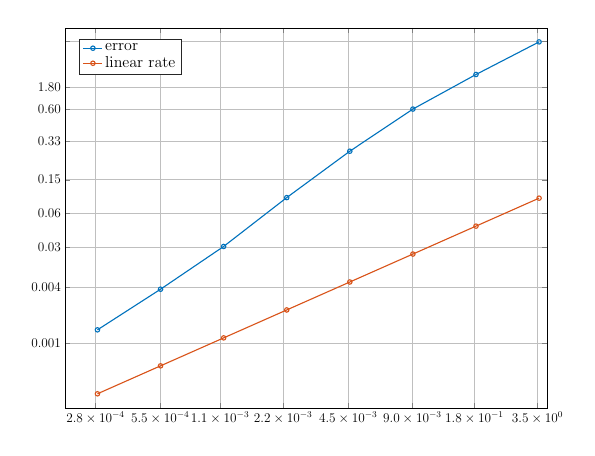
\begin{tikzpicture}[scale=0.4]
\definecolor{mycolor1}{rgb}{0.00000,0.44700,0.74100}%
\definecolor{mycolor2}{rgb}{0.85000,0.32500,0.09800}%
\begin{axis}[%
width=6.028in,
height=4.754in,
at={(1.011in,0.642in)},
scale only axis,
xmode=log,
xmin=0.0002,
xmax=0.04,
grid=major,
tick label style={font=\large},
%xminorticks=true,
xtick={0.00028,    0.00057,    0.0011,    0.0022,    0.0045,    0.0091,    0.018,    0.036},
xticklabels={$2.8\times 10^{-4}$,    $5.5\times 10^{-4}$,    $1.1\times 10^{-3}$,    $2.2\times 10^{-3}$,    $4.5\times 10^{-3}$,    $9.0\times 10^{-3}$,    $1.8\times 10^{-1}$,    $3.5\times 10^{0}$},%{-2,-0.5,0,0.5,2},
ytick={0.001,0.004,0.0108,    0.0250,    0.0579,    0.1503,    0.3329,    0.5744,    1.7814},
yticklabels={0.001,0.004,    0.03,    0.06,    0.15,    0.33,    0.60,    1.80},%{-1,0,1},
ymode=log,
ymin=0.0002,
ymax=2.5,
yminorticks=true,
legend pos=north west,
legend style={font=\Large, legend cell align=left, draw=white!15!black, scale=1},
axis background/.style={fill=white}
]
\addplot [color=mycolor1, line width=1.0pt, mark=o, mark options={solid, mycolor1,scale=1}] %[color=mycolor8, line width=1.0pt, mark=*, mark options={solid, mycolor8,scale=0.15}]
  table[row sep=crcr]{%
 0.036611652351682   1.765887651538395\\
   0.018305826175841   0.786958041220327\\
   0.009152913087920   0.333844052710593\\
   0.004576456543960   0.117332328056215\\
   0.002288228271980   0.037133887036001\\
   0.001144114135990   0.011050624438639\\
   0.000572057067995   0.003825890069851\\
   0.000286028533998   0.001397145327629\\
   };
\addlegendentry{error}
\addplot [color=mycolor2,  mark=o,line width=1.0pt]
  table[row sep=crcr]{%
0.0366116523516816	0.0366116523516816\\
0.0183058261758408	0.0183058261758408\\
0.00915291308792039	0.00915291308792039\\
0.0045764565439602	0.0045764565439602\\
0.0022882282719801	0.0022882282719801\\
0.00114411413599005	0.00114411413599005\\
0.000572057067995024	0.000572057067995024\\
0.000286028533997512	0.000286028533997512\\};
\addlegendentry{linear rate}
\end{axis}

\end{tikzpicture} 
%		\caption{Experimental rate of convergence compared with linear rate}
%		\label{fig:1}
%	\end{figure}
\captionsetup{font=footnotesize}
\captionof{figure}{Experimental error of the optimal control for $q=0.9$}
\label{fig:error q09}
\end{minipage}
\hspace{-3mm}
\begin{minipage}{0.5\textwidth}
\footnotesize
%\begin{table}\label{tab:error1}
\centering
\begin{tabular}{ccccc}
\hline
$h$ &$\|\tilde y_h -\bar y\|_{L^2}$ & EOC & $\|\tilde u_h -\bar u\|_{L^2}$ & EOC \\
\hline\hline
0.0366 & 0.0518 & 1.78 & 1.7658 & 1.23 \\\hline
0.0183 & 0.0081 & 1.67 & 0.7869 & 1.24 \\\hline
0.0092 & 0.0018 & 1.59 & 0.3338 & 1.24 \\\hline
0.0046 & 0.0006 & 1.61 & 0.1173 & 1.19 \\\hline
0.0023 & 0.0002 & 1.58& 0.0371 & 1.10 \\\hline
0.0011 &  0.0001 & 1.37 &0.0110 & 0.94 \\\hline
0.0006 &  $1.3\times 10^{-5}$& 1.01 & 0.0038 & 0.80 \\\hline
%0.0003 &  $3\times 10^{-6 }$& &0.0014 & 0.95 
\end{tabular}
%\end{table}
\captionsetup{font=footnotesize}
\captionof{table}{Experimental order of convergence for  $q=0.9$} 
\label{tab:q09}
\end{minipage}





\begin{minipage}{0.5\textwidth}
%\begin{figure}[ht!]
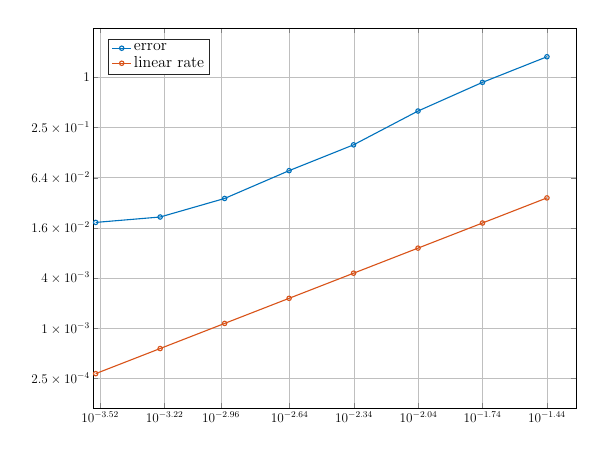
\begin{tikzpicture}[scale=0.4]
\definecolor{mycolor1}{rgb}{0.00000,0.44700,0.74100}%
\definecolor{mycolor2}{rgb}{0.85000,0.32500,0.09800}%
\begin{axis}[%
width=6.028in,
height=4.754in,
at={(1.011in,0.642in)},
scale only axis,
xmode=log,
xmin=0.00028,
xmax=0.05,
grid=major,
tick label style={font=\large},
%xminorticks=true,
xtick={0 ,   0.0003 ,   0.0006,    0.0011 ,   0.0023 ,   0.0046,    0.0092 ,   0.0183 ,   0.0366},
%xticklabels={0 ,   0.0040,    0.0080 ,   0.0120 ,   0.0160 ,   0.0200 ,   0.0240 ,   0.0280 ,   0.0320,    0.0360,    0.04},%{-2,-0.5,0,0.5,2},
ytick={ 0.00025, 1e-3,0.004, 0.016,   0.0640  ,  0.2560  , 1.0240},
yticklabels={$2.5\times 10^{-4}$, $1\times 10^{-3}$,  $4\times 10^{-3}$,  $1.6\times 10^{-2}$,   $6.4\times 10^{-2}$ ,    $2.5\times 10^{-1}$,    1},%{-1,0,1},
ymode=log,
ymin=0.0,
ymax=4,
yminorticks=true,
legend pos=north west,
legend style={font=\Large, legend cell align=left, draw=white!15!black, scale=1},
axis background/.style={fill=white}
]
\addplot [color=mycolor1, line width=1.0pt, mark=o, mark options={solid, mycolor1,scale=1}] %[color=mycolor8, line width=1.0pt, mark=*, mark options={solid, mycolor8,scale=0.15}]
  table[row sep=crcr]{%
0.036611652351682   1.803381576744028\\
   0.018305826175841   0.889253802037622\\
   0.009152913087920   0.403049642353783\\
   0.004576456543960   0.158492196915685\\
   0.002288228271980   0.077685528057962\\
   0.001144114135990   0.036041303168884\\
   0.000572057067995   0.021601994699690\\
   0.000286028533998   0.018605157286952\\
};
\addlegendentry{error}
\addplot [color=mycolor2,  mark=o,line width=1.0pt]
  table[row sep=crcr]{%
   0.036611652351682   0.036611652351682\\
   0.018305826175841   0.018305826175841\\
   0.009152913087920   0.009152913087920\\
   0.004576456543960   0.004576456543960\\
   0.002288228271980   0.002288228271980\\
   0.001144114135990   0.001144114135990\\
   0.000572057067995   0.000572057067995\\
   0.000286028533998   0.000286028533998\\
   };
\addlegendentry{linear rate}
\end{axis}

\end{tikzpicture} 
%		\caption{Experimental rate of convergence compared with linear rate}
%		\label{fig:1}
%	\end{figure}
\captionsetup{font=footnotesize}
\captionof{figure}{Experimental error of the optimal control for $q=0.5$}
\label{fig:error q05}
\end{minipage}
\hspace{-3mm}
\begin{minipage}{0.5\textwidth}
\footnotesize
%\begin{table}\label{tab:error1}
\centering
\begin{tabular}{ccccc}
\hline
$h$ &$\|\tilde y_h -\bar y\|_{L^2}$ & EOC & $\|\tilde u_h -\bar u\|_{L^2}$ & EOC \\
\hline\hline
0.0366 & 0.0552 & 1.60 & 1.8033 & 1.02 \\\hline
0.0183 & 0.0082 & 1.46   & 0.8892 & 1.03 \\\hline
0.0092 & 0.0022 & 1.41   & 0.4030 &1.01 \\\hline
0.0046 & 0.0014 & 1.53   & 0.1584 & 0.95 \\\hline
0.0023 & 0.0002 & 1.30  & 0.0776&0.94 \\\hline
0.0011 & $1.1\times 10^{-4}$ & 1.39& 0.0360& 0.89 \\\hline
0.0006 & $3\times 10^{-5}$& 1.13&0.0216& 0.95 \\\hline
0.0003 & $8\times 10^{-6}$& 0.90 &0.0186 & 1.30
\end{tabular}
%\end{table}
\captionsetup{font=footnotesize}
\captionof{table}{Experimental error of convergence  $q=0.5$} 
\label{tab:q05}
\end{minipage}

\begin{minipage}{0.5\textwidth}
%\begin{figure}[ht!]
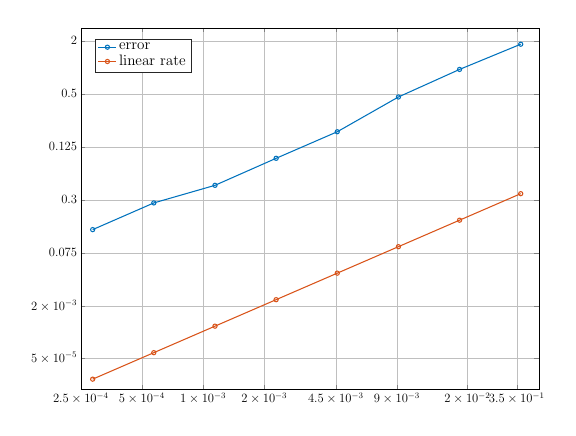
\begin{tikzpicture}[scale=0.38]
\definecolor{mycolor1}{rgb}{0.00000,0.44700,0.74100}%
\definecolor{mycolor2}{rgb}{0.85000,0.32500,0.09800}%
\begin{axis}[%
width=6.028in,
height=4.754in,
at={(1.011in,0.642in)},
scale only axis,
xmode=log,
xmin=0.00025,
xmax=0.045,
grid=major,
tick label style={font=\large},
%xminorticks=true,
xtick={0.00025, 0.0005,    0.001,    0.002,    0.0045,    0.009,    0.02,    0.035},
xticklabels={$2.5\times 10^{-4}$,    $5\times 10^{-4}$,    $1\times 10^{-3}$,    $2\times 10^{-3}$,    $4.5\times 10^{-3}$,    $9\times 10^{-3}$,    $2\times 10^{-2}$,    $3.5\times 10^{-1}$},%{-2,-0.5,0,0.5,2},
ytick={ 0.0005,    0.001953,    0.0078125,    0.03125,    0.125,    0.5,    2},
yticklabels={ $5\times 10^{-5}$,    $2\times 10^{-3}$,    0.075,    0.3,    0.125,    0.5,    2},%{-1,0,1},
ymode=log,
ymin=0.00022,
ymax=2.8,
yminorticks=true,
legend pos=north west,
legend style={font=\Large, legend cell align=left, draw=white!15!black, scale=1},
axis background/.style={fill=white}
]
\addplot [color=mycolor1, line width=1.0pt, mark=o, mark options={solid, mycolor1,scale=1}] %[color=mycolor8, line width=1.0pt, mark=*, mark options={solid, mycolor8,scale=0.15}]
  table[row sep=crcr]{%
   0.036611652351682   1.826883886305578\\
   0.018305826175841   0.944773344431918\\
   0.009152913087920   0.459359193791866\\
   0.004576456543960   0.184979175198573\\
   0.002288228271980   0.092376089968164\\
   0.001144114135990   0.045553412495355\\
   0.000572057067995   0.028743807751765\\
   0.000286028533998   0.014299868037441\\};
\addlegendentry{error}
\addplot [color=mycolor2,  mark=o,line width=1.0pt]
  table[row sep=crcr]{%
0.0366116523516816	0.0366116523516816\\
0.0183058261758408	0.0183058261758408\\
0.00915291308792039	0.00915291308792039\\
0.0045764565439602	0.0045764565439602\\
0.0022882282719801	0.0022882282719801\\
0.00114411413599005	0.00114411413599005\\
0.000572057067995024	0.000572057067995024\\
0.000286028533997512	0.000286028533997512\\};
\addlegendentry{linear rate}
\end{axis}
\end{tikzpicture} 
%		\caption{Experimental rate of convergence compared with linear rate}
%		\label{fig:1}
%	\end{figure}
\captionsetup{font=footnotesize}
\captionof{figure}{Experimental error of the optimal control for $q=0.1$}
\label{fig:error q01}
\end{minipage}
%
\hspace{-3mm}
\begin{minipage}{0.5\textwidth}
\footnotesize
%\begin{table}\label{tab:error1}
\centering
\begin{tabular}{ccccc}
\hline
$h$ &$\|\tilde y_h -\bar y\|_{L^2}$ & EOC & $\|\tilde u_h -\bar u\|_{L^2}$ & EOC \\
\hline\hline
0.0366 & 0.05699 & 1.48 & 1.8268 & 0.96 \\\hline
0.0183 & 0.00793 & 1.31 &0.9447 & 0.96 \\\hline
0.0092 & 0.00190 & 1.20 &0.4593 & 0.95 \\\hline
0.0046 & 0.00101 & 1.25 &0.1849 & 0.89 \\\hline
0.0023 & 0.00023 & 1.09 &0.0923 & 0.87 \\\hline
0.0011 & 0.00014 & 1.18 &0.0455 & 0.83 \\\hline
0.0006 & 0.00003& 0.87 &0.0287 & 0.89 \\\hline
0.0003 & 0.00002& 0.94 &0.0142 & 0.83 \\\hline
\end{tabular}
%\end{table}
\captionsetup{font=footnotesize}
\captionof{table}{Experimental order of convergence (EOC) for  $q=0.1$} 
\label{tab:q01}
\end{minipage}
